\section{Experimental Results}
\label{sec:exp}

We conduct various experiments to evaluate our proposed method.
%The datasets are publicly available at the SNAP website.\footnote{http://snap.stanford.edu/data/index.html}

\subsection{Experiment 1}

\begin{table}[t]
\centering
\begin{tabular}{|c|c@{ }|c@{ }|}
\hline
Dataset             &   \#nodes       &   \#edges \\ \hline
aut-as19971108 & 3015 & 5156 \\\hline
aut-as19990628 & 5322 & 10163 \\\hline
cit-scimet & 3085 & 13474 \\\hline
col-ca-GrQc & 5242 & 14484 \\\hline
col-netscience & 1461 & 2742 \\\hline
met-HI & 1424 & 3423 \\\hline
ppi-ppiall & 3258 & 12930 \\\hline
ppi-ppiapms & 1622 & 9070 \\\hline
pwr-power & 4941 & 6594 \\\hline
\end{tabular}
\caption{Statistics of the nine networks.}
\label{tb:statistics}
\end{table}


\vpara{Data sets.} We evaluate the proposed method on nine different networks: aut-as19971108, aut-as19990628, cit-scimet, col-ca-GrQc, col-netscience, met-HI, ppi-ppiall, ppi-ppiapms and pwr-power.
Table \ref{tb:statistics} lists statistics of the nine networks.  All data was obtained from Jure Leskovec at Stanford University.

\vpara{Evaluation metrics.} To quantitatively evaluate the proposed model, we use the average relative error between the model's motif counts and the motif counts of the real network.  The average relative error is defined in equation~\ref{eqn:avgRelativeError}.

All code is implemented in C++ and Python, and all the evaluations are performed on an x64 machine with Xeon E7-8837 CPU (with 64 cores) and 1024GB RAM. The operating system is CentOS 6. 

\vpara{Performance analysis.}
Hill climbing produces excellent results on most networks.  Table ~\ref{table:errors} shows the improvements in the error after running hill climbing for 24 hours.

Although performance varies across networks, we get at least a 50\% decrease in error for all networks except aut-as19990628 and cit-scimet.  For some networks we get an enormous reduction in error; pwr-power gives a 99.5\% reduction and met-HI gives a 99.9\% reduction.  The first group of figures plots the error over time and the second group plots the probability that a rewiring step will be successful (i.e. that the changes are accepted instead of discarded).

The error graphs for aut-as19971108 (Figure~\ref{fig:errors-aut-as19971108}) and col-netscience (Figure~\ref{fig:errors-col-netscience}) converge to an asymptote.  This indicates that running the procedure longer would not improve the error and the final error is a good reflection of the algorithm's performance.  Since the errors approach nonzero values (and we know a perfect solution exists), this implies that our hill climbing algorithm has found a local minimum.

The graph for pwr-power (Figure~\ref{fig:errors-pwr-power}) rapidly decreases to zero.  This means we have found a perfect or near-perfect solution.  The graph for met-HI (Figure~\ref{fig:errors-met-HI}) also appears to decrease to zero, but that's just because the error started out very high.  (The initial error was 8039.58 and the final error was 0.46768.)

The other error graphs have not yet converged and are steadily decreasing 24 hours after the computation.  This indicates that we can reduce the final error by increasing the computation time and our current results are not a hard limit on the algorithm's performance.

%In order to quantify the algorithm's convergence, we plotted the successful rewiring probability over time.  This is the probability that rewiring two edges produces a graph with smaller error than the previous graph.  When this probability reaches zero, the hill climbing algorithm has found a local minimum and cannot proceed further.

%The probability curves for pwr-power (Figure~\ref{fig:Paccept-pwr-power}) and col-netscience (Figure~\ref{fig:Paccept-col-netscience}) quickly drop to zero, indicating that the algorithm has converged.  The curves for cit-scimet (Figure~\ref{fig:Paccept-cit-scimet}) and aut-as19990628 (Figure~\ref{fig:Paccept-aut-as19990628}) remain high throughout the algorithm, indicating that we need to run the algorithm longer.  The other curves do not drop to zero, but hover at small nonzero values.  This means the algorithm has not yet converged, but running it longer may yield diminishing returns.

\begin{table*}[t]
\centering
\begin{tabular}{| l | l | l | | l | l | l |}
\hline
Network & Nodes & Edges & Initial error & Final error & Successful rewires\\ \hline
aut-as19971108 & 3015 & 5156 & 0.34216 & 0.16717 & 2951.00\\\hline
aut-as19990628 & 5322 & 10163 & 0.31571 & 0.17723 & 3397.28\\\hline
cit-scimet & 3085 & 13474 & 0.83063 & 0.73247 & 1921.71\\\hline
col-ca-GrQc & 5242 & 14484 & 2.05549 & 0.93973 & 40583.8\\\hline
col-netscience & 1461 & 2742 & 3.13864 & 0.55110 & 8290.71\\\hline
met-HI & 1424 & 3423 & 8039.58 & 0.46768 & 5703.57\\\hline
ppi-ppiall & 3258 & 12930 & 1.06249 & 0.46058 & 38131.1\\\hline
ppi-ppiapms & 1622 & 9070 & 1.37580 & 0.54219 & 24581.7\\\hline
pwr-power & 4941 & 6594 & 0.57996 & 0.00282 & 9485.4\\\hline
\end{tabular}
\caption{Improvements in error after running hill climbing for 24 hours.  All numbers are averaged over $7$ trials.}
\label{table:errors}
\end{table*}

\subsection{Experiment 2}

\vpara{Experimental setup.}
In our second experiment we made three changes.

\begin{enumerate}
\item We ran the simulation for 3.66 days instead of 24 hours.
\item We used a slower library function to generate the initial graph.  
The original function generated a random graph with approximately 
the same degree distribution as the real-world graph, but the new 
function uses the exact degree distribution.
\item We plotted the relative error for each motif, which we defined as
$$\frac{|count - \widehat{count}|}{count}.$$  For brevity, only a
few of these plots are shown here.
\end{enumerate}

\vpara{Performance analysis.}
Although performance varies across networks (Table~\ref{table:errors-exp2}), 
we get at least a 58\% decrease in error for each of the networks, and at 
least an 84\% decrease for all networks except ppi-ppiapms.  The first
group of figures plots the error over time, where only successful rewiring
steps are plotted.

The error for ppi-ppiapms (Figure~\ref{fig:exp2-ppi-ppiapms-run}) does not
approach a horizontal asymptote, indicating that increasing the
computation time would improve the error.

The errors for col-ca-GrQc (Figure~\ref{fig:exp2-col-ca-GrQc-run}) and
col-netscience (Figure~\ref{fig:exp2-col-netscience-run}) do approach a
horizontal asymptote, which means the algorithm has reached a
local minimum.  This means we should use other techniques to improve
the error, such as simulated annealing, MCMC, or the method of random
restarts.

The error for pwr-power (Figure~\ref{fig:exp2-pwr-power-run}) converges to 
0.006.  Although this error was nonzero and probably a local minimum, we 
can still say the algorithm was successful because the error was very small.

On the met-HI network (Figure~\ref{fig:exp2-met-HI-run}), the motif 
counts of the generated graph were identical to the
desired motif counts.  The error is 0.4 because we added $1$ to the
numerator and denominator of the error function to avoid dividing by zero
(Equation~\ref{eqn:avgRelativeError}).  In Experiment 3, we changed the
error function to avoid this issue (Equation~\ref{eqn:newErrorFunction}).

\vpara{Error for each motif.}  We plot the per-motif errors for pwr-power
in Figures~\ref{fig:exp2-pwr-power-mfFourComplete},
\ref{fig:exp2-pwr-power-mfFourLine},
\ref{fig:exp2-pwr-power-mfFourSquare},
\ref{fig:exp2-pwr-power-mfFourSquareDiag},
\ref{fig:exp2-pwr-power-mfFourStar},
\ref{fig:exp2-pwr-power-mfFourTriangleEdge},
\ref{fig:exp2-pwr-power-mtThreeClosed}, and
\ref{fig:exp2-pwr-power-mtThreeOpen}.
In this network most motif errors steadily decrease to zero.  However, the
Four Line motif error decreases to zero and then rises again
(Figure~\ref{fig:exp2-pwr-power-mfFourLine}).  The rise
appears concurrently with changes in the other plots.  At this point,
the Four Square Diag error becomes zero
(Figure~\ref{fig:exp2-pwr-power-mfFourSquareDiag}) and the Four Star curve
becomes a lot flatter.  We suspect that the rise marks a single rewiring
step that greatly affected the topology of the graph.  This might have 
happened if an edge involved was connected with many motifs.

\begin{table*}[t]
\centering
\begin{tabular}{| l | l | l | | l | l | l |}
\hline
Network & Nodes & Edges & Initial error & Final error & Successful rewires\\ \hline
col-ca-GrQc & 5242 & 14484 & 5.13635& 0.83224& 63925 \\\hline
col-netscience & 1461 & 2742 & 7.63883& 0.59894& 8048 \\\hline
met-HI & 1424 & 3423 & 19129.09& 0.40010& 5109 \\\hline
ppi-ppiapms & 1622 & 9070 & 1.57338& 0.67426& 30160 \\\hline
pwr-power & 4941 & 6594 & 0.58720& 0.00596& 14324 \\\hline
\end{tabular}
\caption{Improved hill climbing and ran it for 3.66 days.}
\label{table:errors-exp2}
\end{table*}

\subsection{Preliminary results: random restarts}
In our third experiment we implemented the method of random restarts.  Due
to time constraints we only ran the method on the small graph pro-polbooks.
Since our old error function did not produce zero error on correct motif
counts, we changed the error function to

\begin{eqnarray}
\label{eqn:newErrorFunction}
\mbox{Average relative error} = \frac{1}{\ell} \sum_{i = 1}^{\ell} \mbox{error}_i\nonumber\\
\mbox{error}_i = |\mbox{counts}_i - \widehat{\mbox{counts}}_i| \mbox{ if counts}_i = 0\\
\mbox{error}_i = \frac{|\mbox{counts}_i - \widehat{\mbox{counts}}_i|}{\mbox{counts}_i} \mbox{ if counts}_i \neq 0\nonumber
\end{eqnarray}

where $\ell$ is the number of different motif types.

In Table~\ref{tb:random-restarts} we see this result produces $0\%$
improvement over the baseline.  The baseline was calculated by returning
the error at the first local minimum.  In this case the first local minimum
was the best one.  In the future we will try this on more networks and hope
for better results.

\begin{table*}[t]
\centering
\begin{tabular}{|l|l|l|l|l|l|l|l|}
\hline
Dataset & \#Nodes & \#Edges & Successful rewires& Initial error & Best error & Baseline error & Percent improvement \\ \hline
pro-polbooks & 105 & 441 & 190656 & 0.50658 & 0.01129& 0.01129& 0.00000 \\\hline
\end{tabular}
\caption{Method of random restarts.}
\label{tb:random-restarts}
\end{table*}

\begin{figure}[p]
\centering
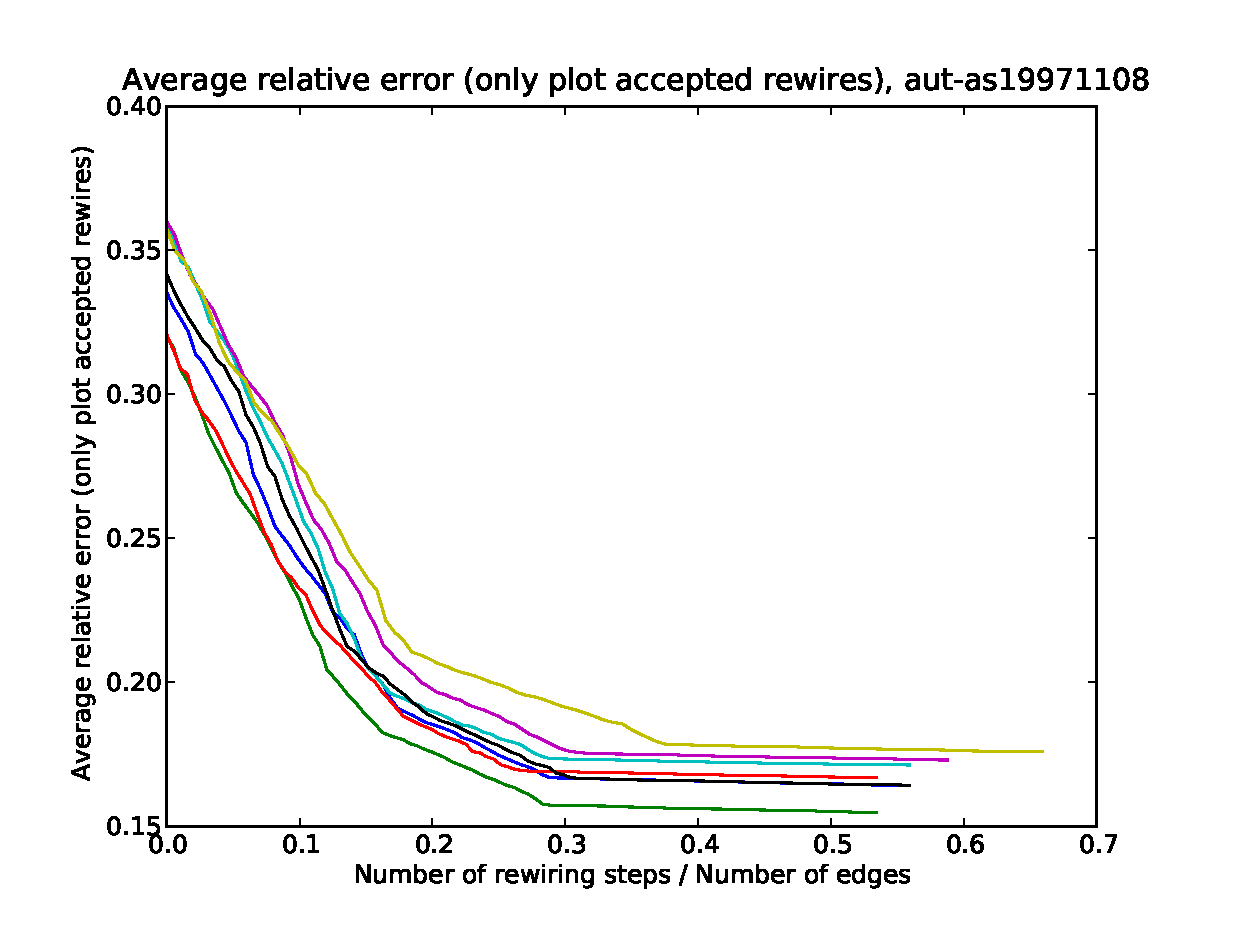
\includegraphics[width=3in]{Figures/acceptedOnly-aut-as19971108.eps}
\caption{Error, network aut-as19971108.  Only plot hill climbing steps that were successful.}
\label{fig:errors-aut-as19971108}
\end{figure}

\begin{figure}[p]
\centering
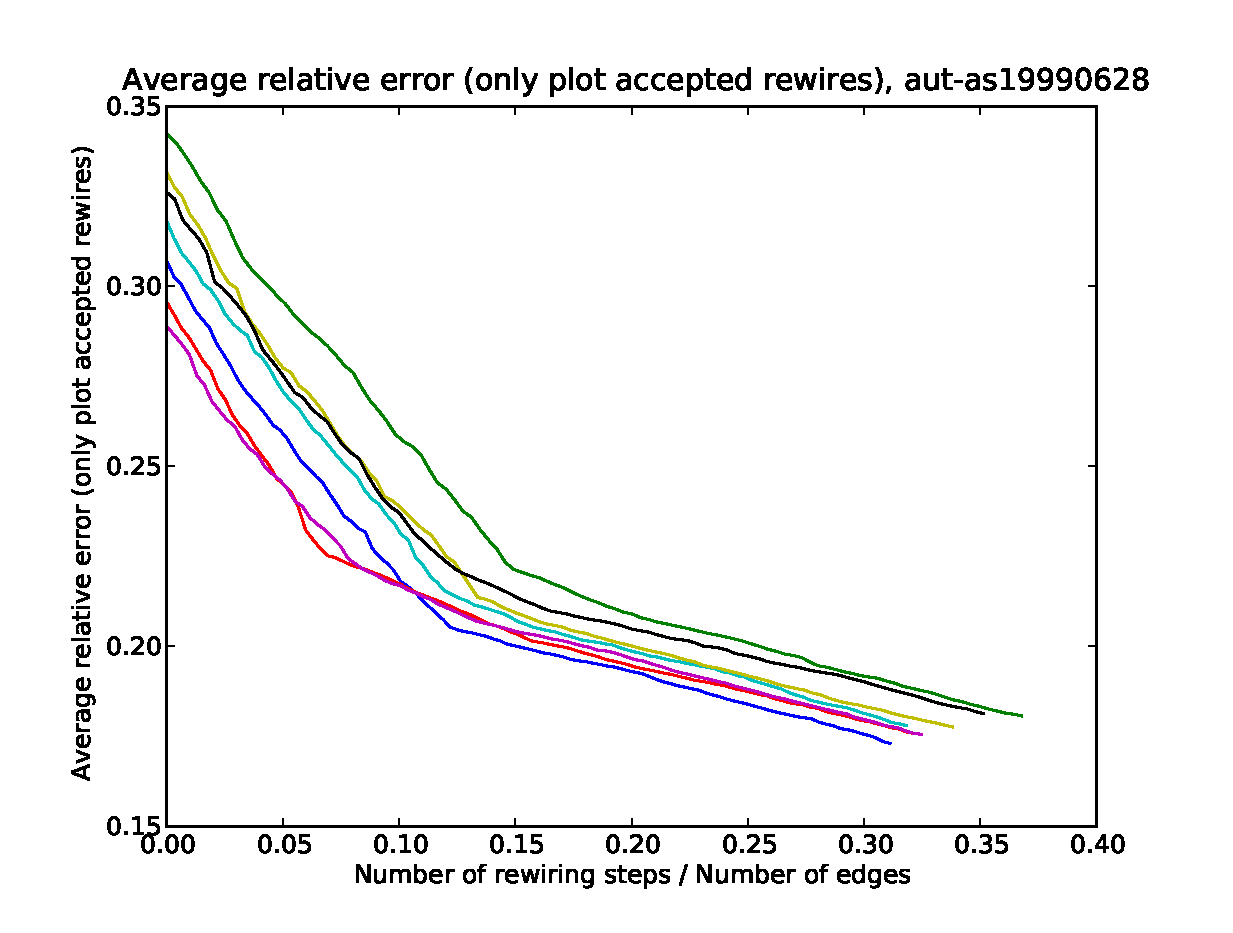
\includegraphics[width=3in]{Figures/acceptedOnly-aut-as19990628.eps}
\caption{Error, network aut-as19990628.  Only plot hill climbing steps that were successful.}
\label{fig:errors-aut-as19990628}
\end{figure}

\begin{figure}[p]
\centering
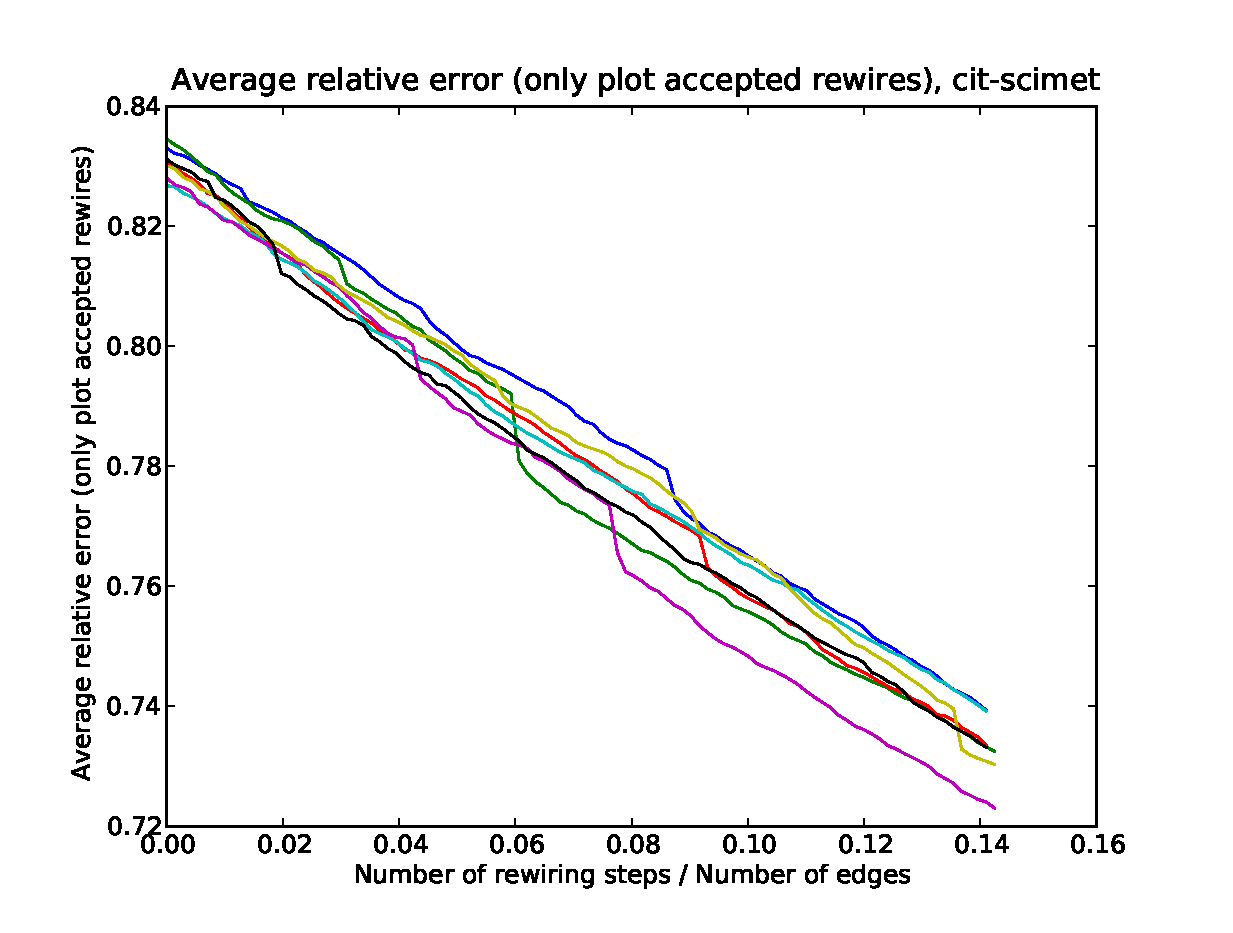
\includegraphics[width=3in]{Figures/acceptedOnly-cit-scimet.eps}
\caption{Error, network cit-scimet.  Only plot hill climbing steps that were successful.}
\label{fig:errors-cit-scimet}
\end{figure}

\begin{figure}[p]
\centering
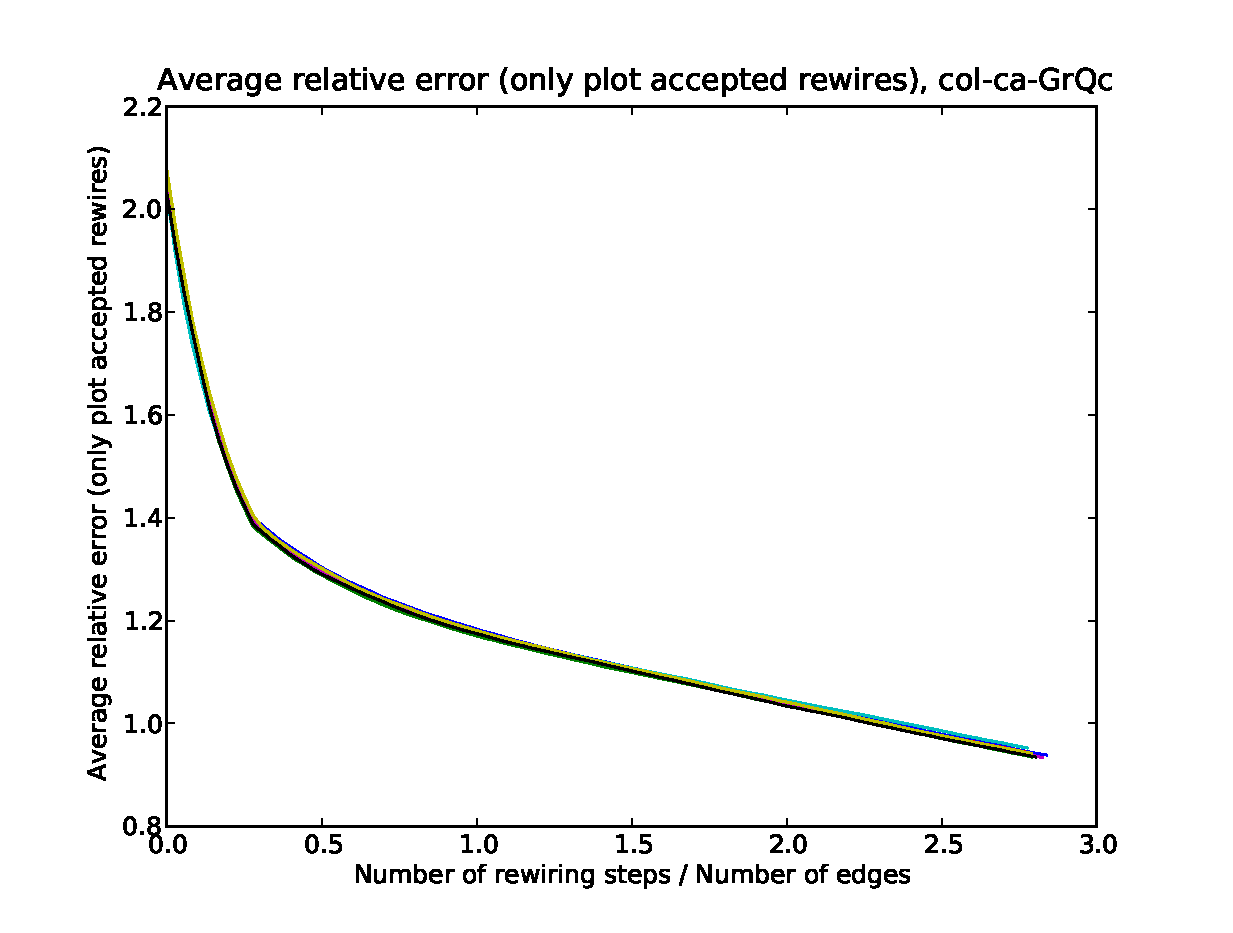
\includegraphics[width=3in]{Figures/acceptedOnly-col-ca-GrQc.eps}
\caption{Error, network col-ca-GrQc.  Only plot hill climbing steps that were successful.}
\label{fig:errors-col-ca-GrQc}
\end{figure}

\begin{figure}[p]
\centering
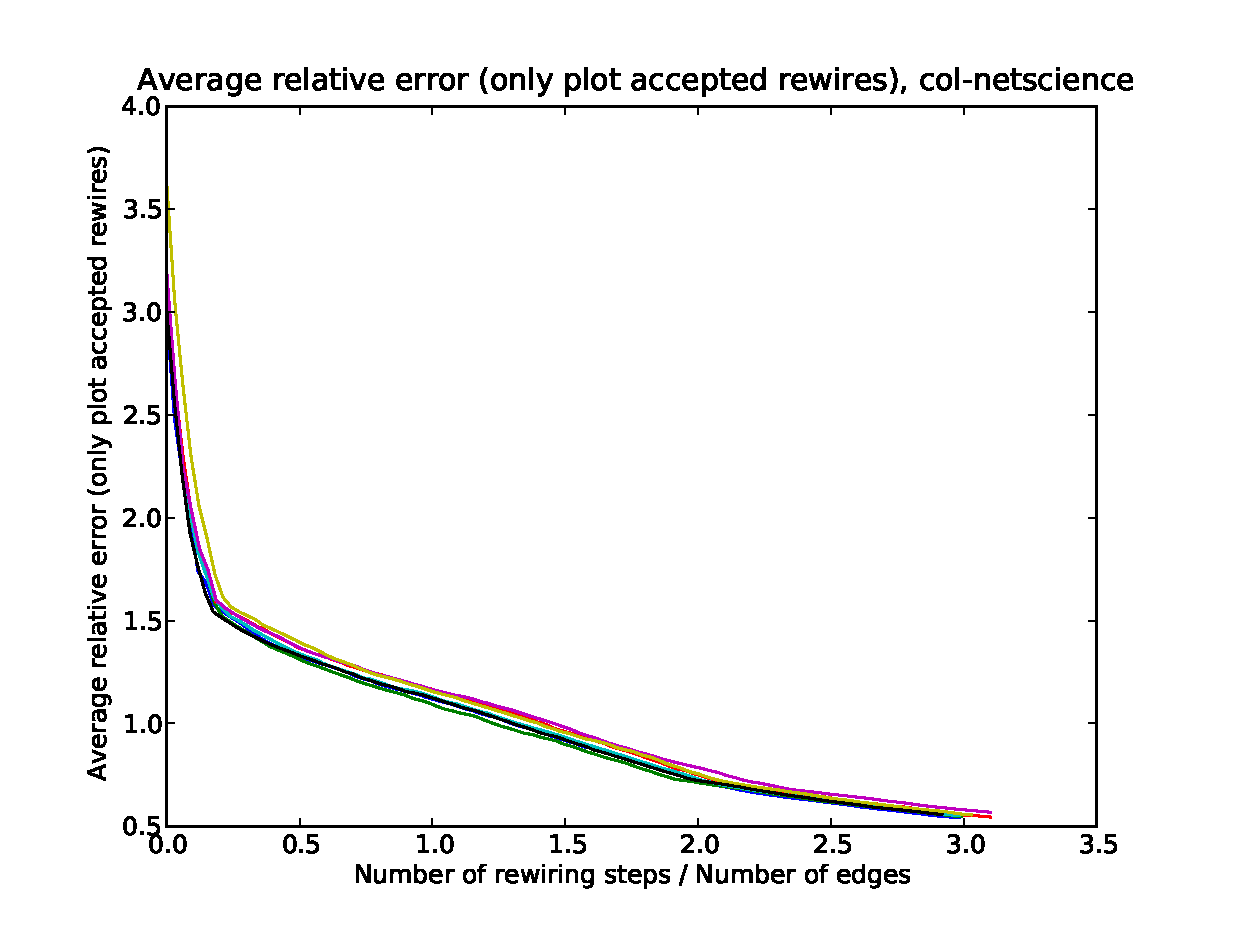
\includegraphics[width=3in]{Figures/acceptedOnly-col-netscience.eps}
\caption{Error, network col-netscience.  Only plot hill climbing steps that were successful.}
\label{fig:errors-col-netscience}
\end{figure}

\begin{figure}[p]
\centering
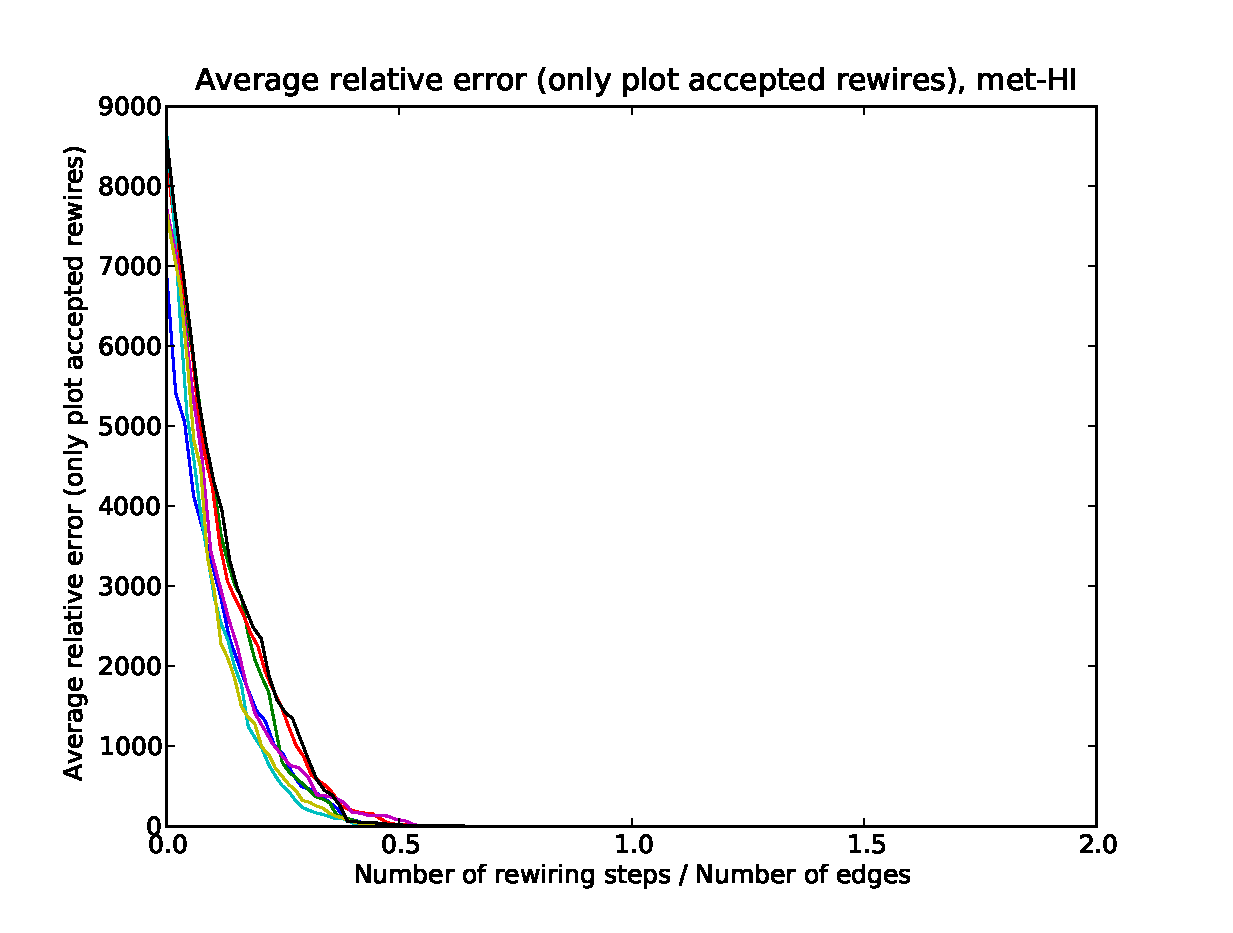
\includegraphics[width=3in]{Figures/acceptedOnly-met-HI.eps}
\caption{Error, network met-HI.  Only plot hill climbing steps that were successful.}
\label{fig:errors-met-HI}
\end{figure}

\begin{figure}[p]
\centering
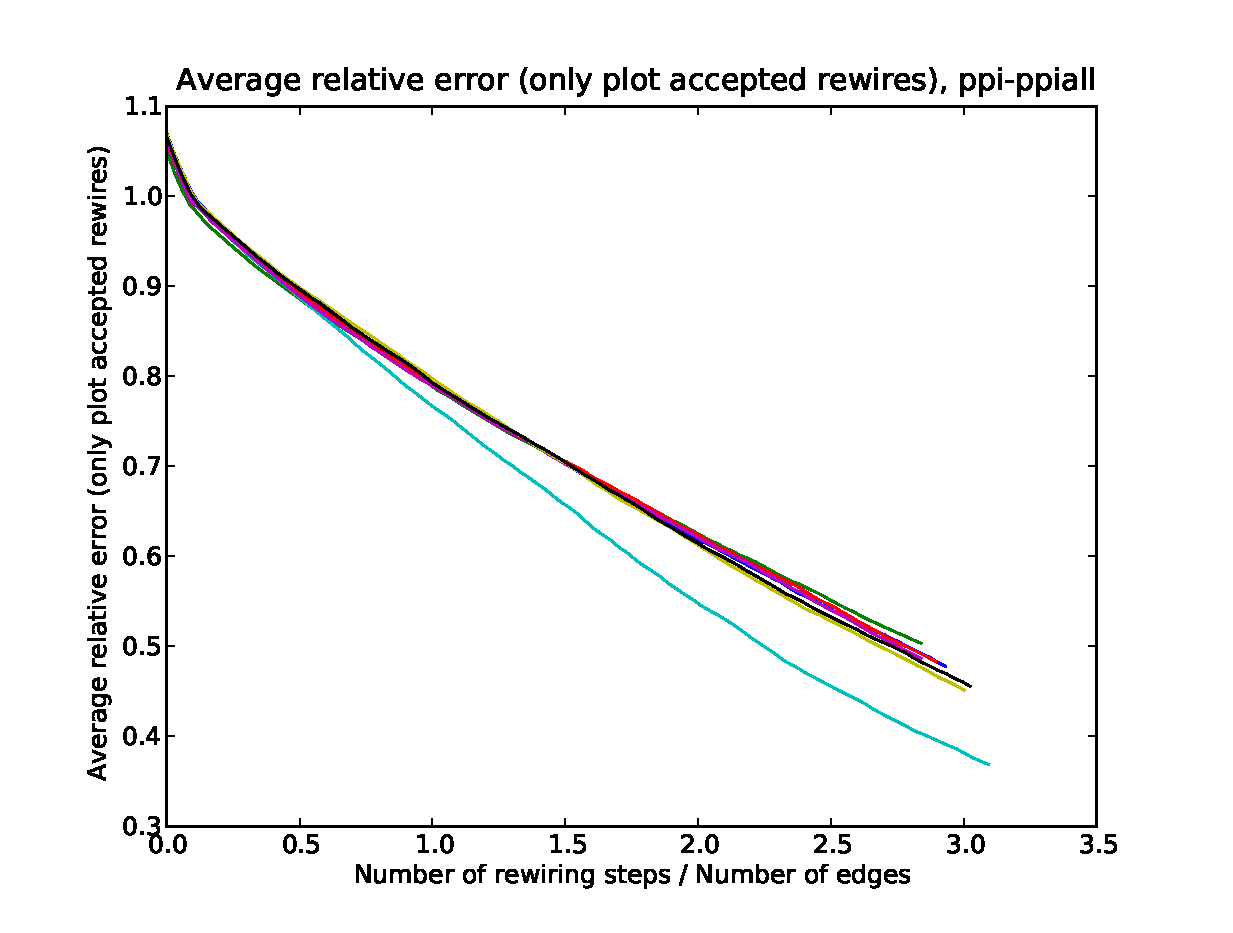
\includegraphics[width=3in]{Figures/acceptedOnly-ppi-ppiall.eps}
\caption{Error, network ppi-ppiall.  Only plot hill climbing steps that were successful.}
\label{fig:errors-ppi-ppiall}
\end{figure}

\begin{figure}[p]
\centering
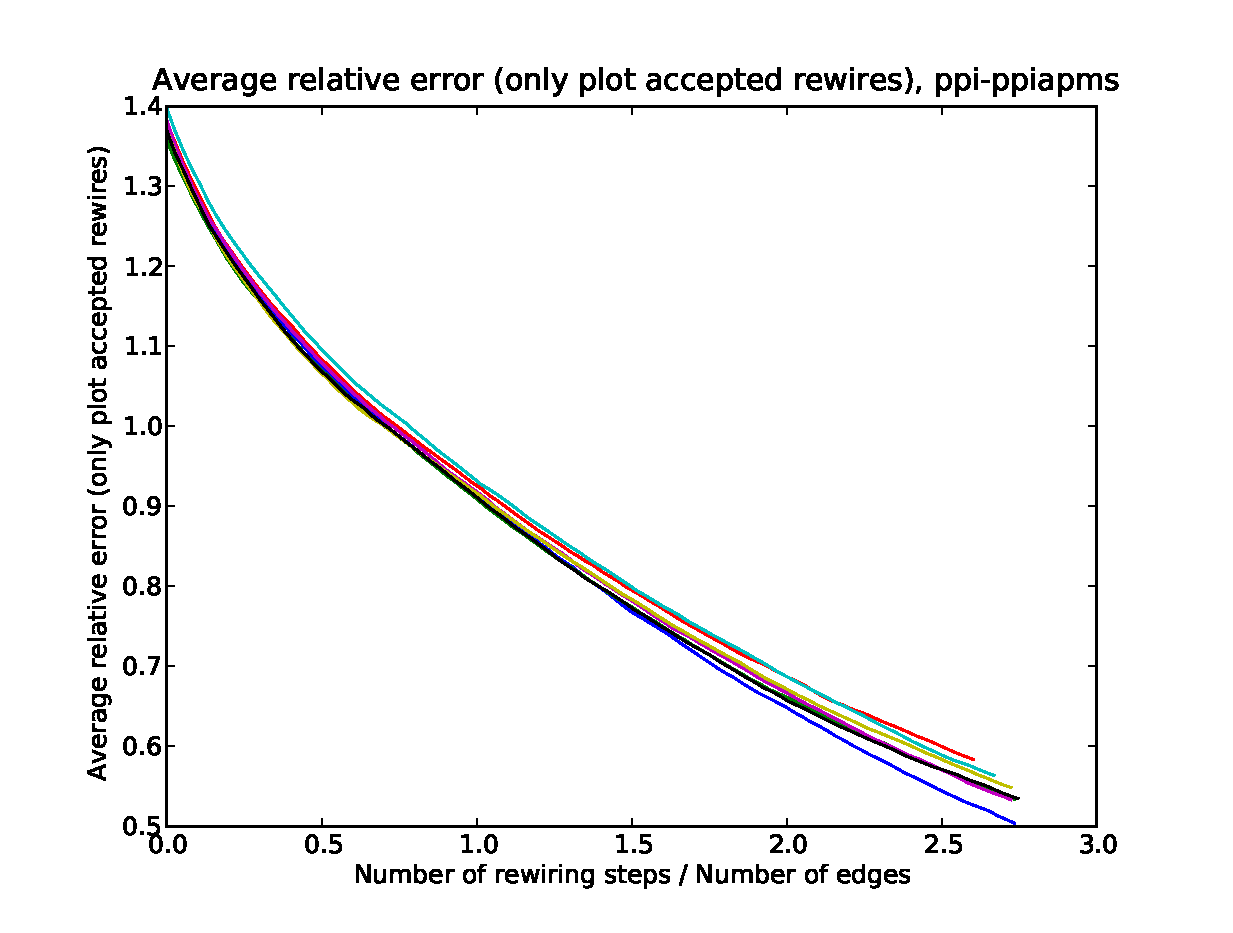
\includegraphics[width=3in]{Figures/acceptedOnly-ppi-ppiapms.eps}
\caption{Error, network ppi-ppiapms.  Only plot hill climbing steps that were successful.}
\label{fig:errors-ppi-ppiapms}
\end{figure}

\begin{figure}[p]
\centering
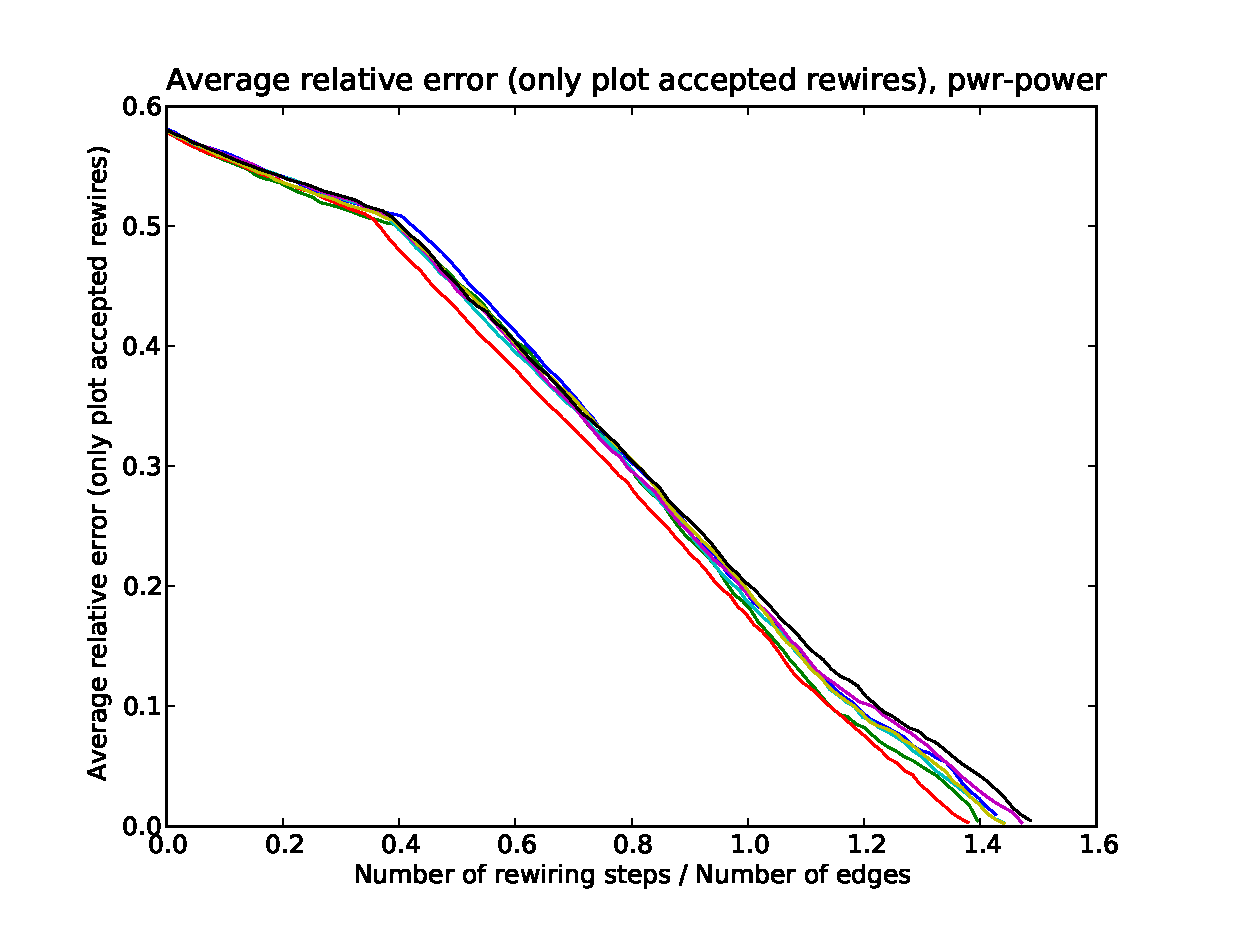
\includegraphics[width=3in]{Figures/acceptedOnly-pwr-power.eps}
\caption{Error, network pwr-power.  Only plot hill climbing steps that were successful.}
\label{fig:errors-pwr-power}
\end{figure}

\begin{figure}[p]
\centering
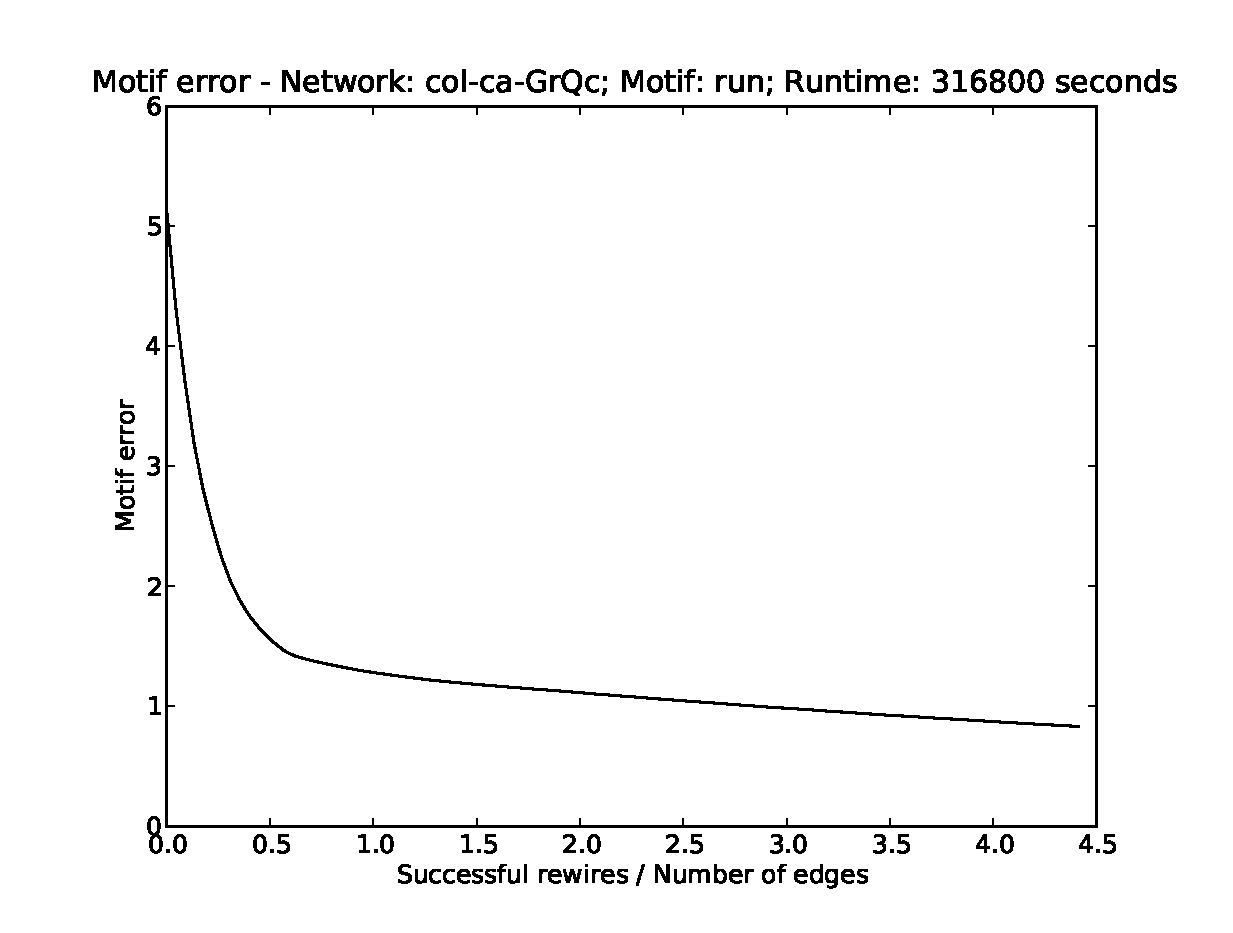
\includegraphics[width=3in]{Figures/motif_error-col-ca-GrQc-run.eps}
\caption{Experiment 2, network col-ca-GrQc.}
\label{fig:exp2-col-ca-GrQc-run}
\end{figure}

\begin{figure}[p]
\centering
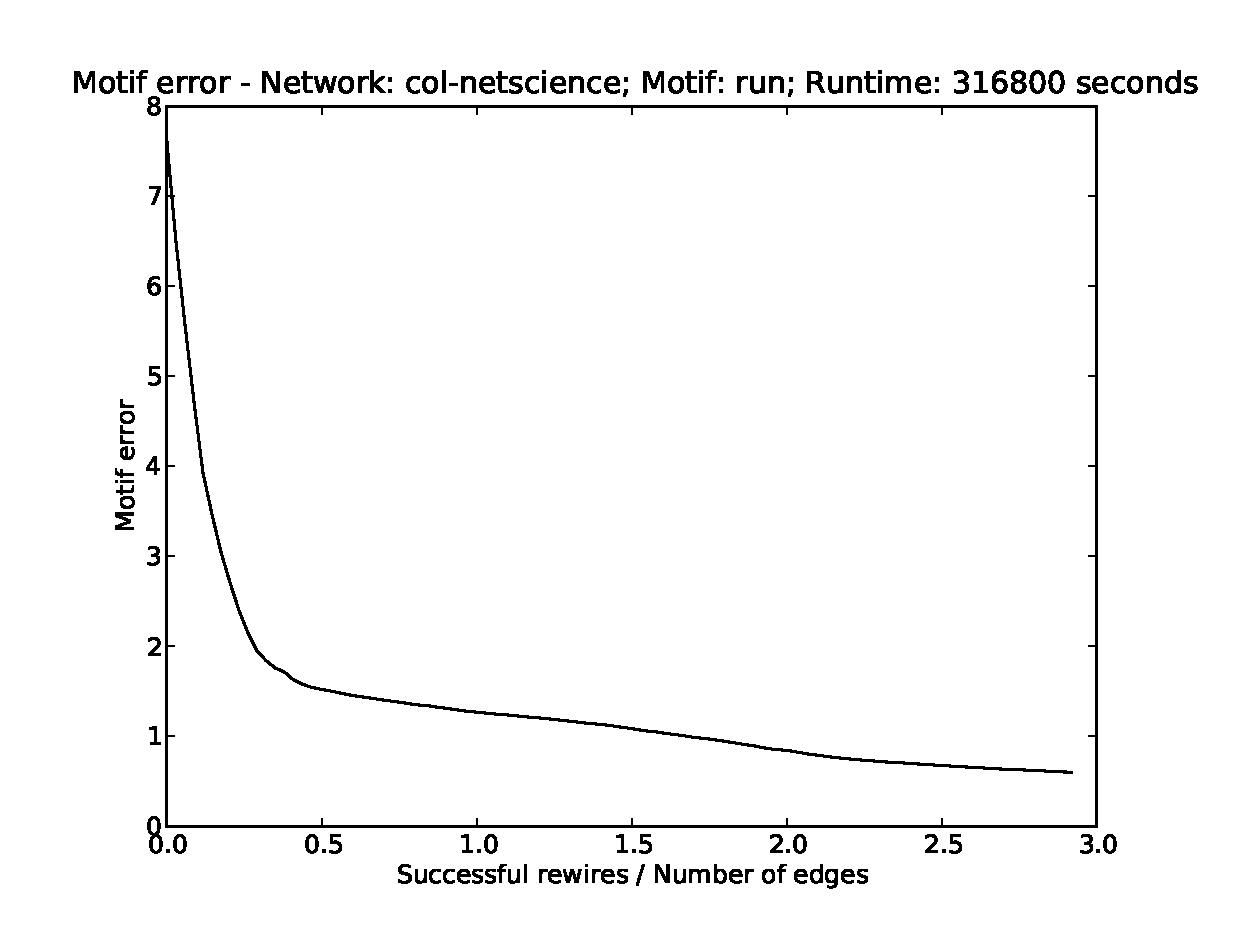
\includegraphics[width=3in]{Figures/motif_error-col-netscience-run.eps}
\caption{Experiment 2, network col-netscience.}
\label{fig:exp2-col-netscience-run}
\end{figure}

\begin{figure}[p]
\centering
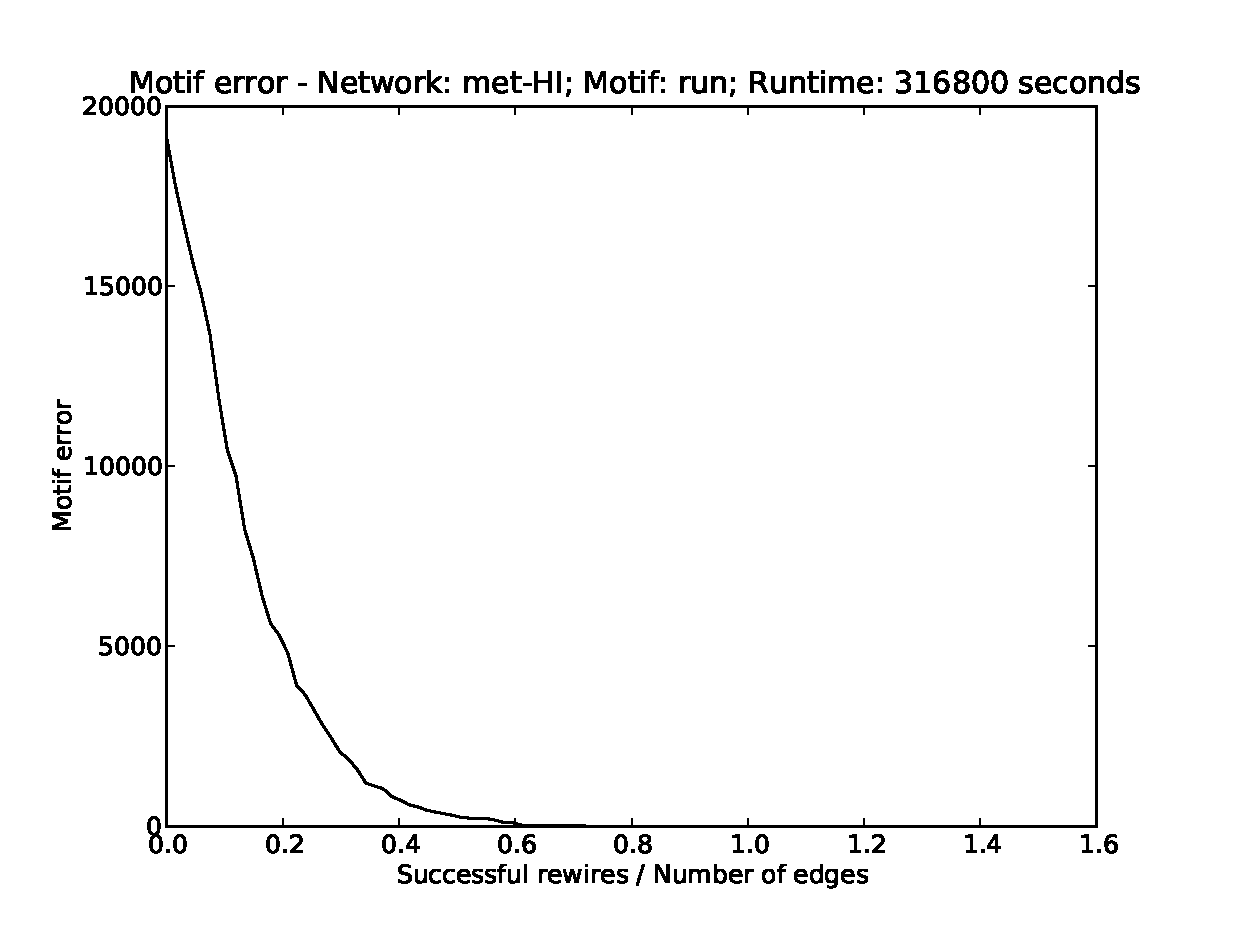
\includegraphics[width=3in]{Figures/motif_error-met-HI-run.eps}
\caption{Experiment 2, network met-HI.}
\label{fig:exp2-met-HI-run}
\end{figure}

\begin{figure}[p]
\centering
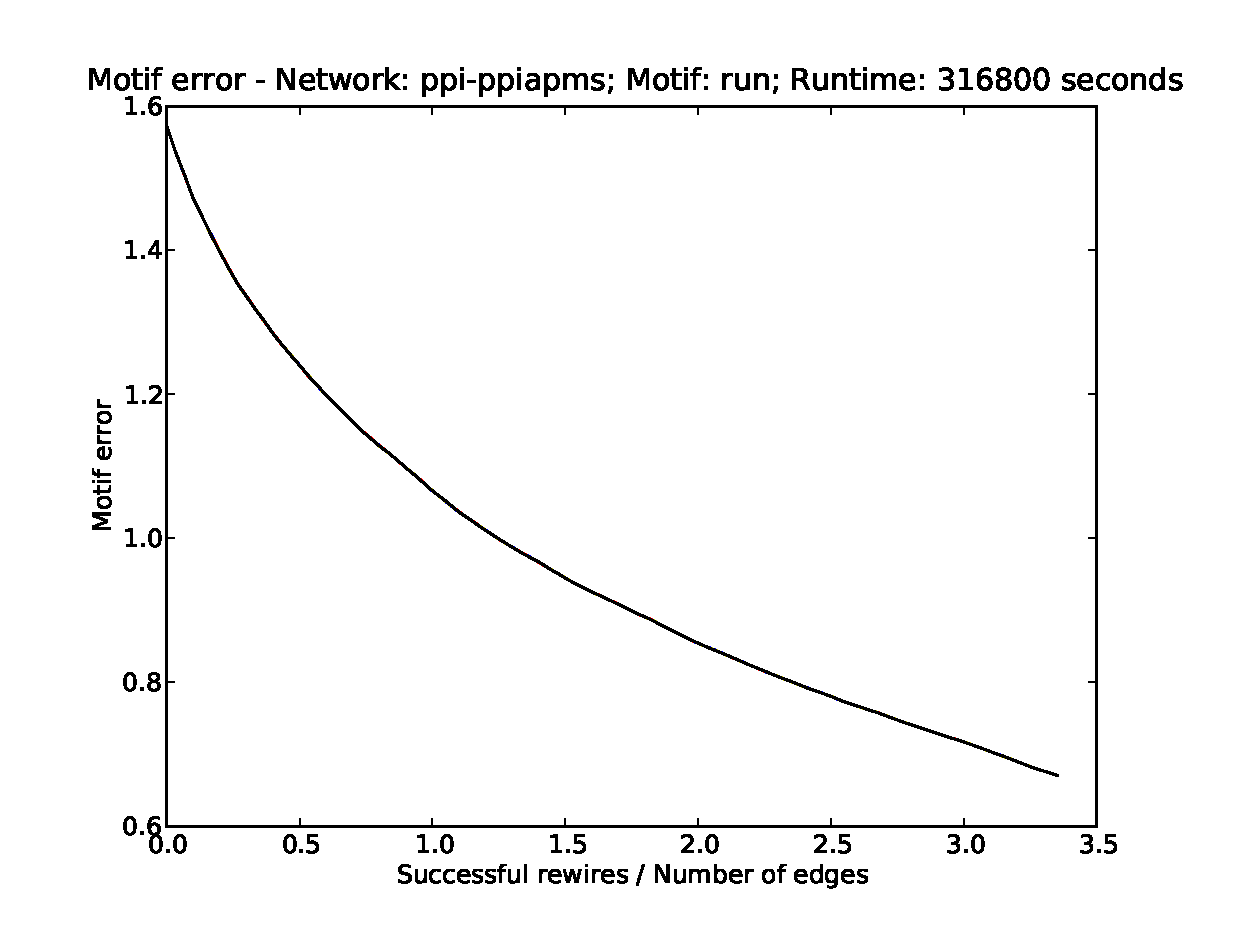
\includegraphics[width=3in]{Figures/motif_error-ppi-ppiapms-run.eps}
\caption{Experiment 2, network ppi-ppiapms.}
\label{fig:exp2-ppi-ppiapms-run}
\end{figure}

\begin{figure}[p]
\centering
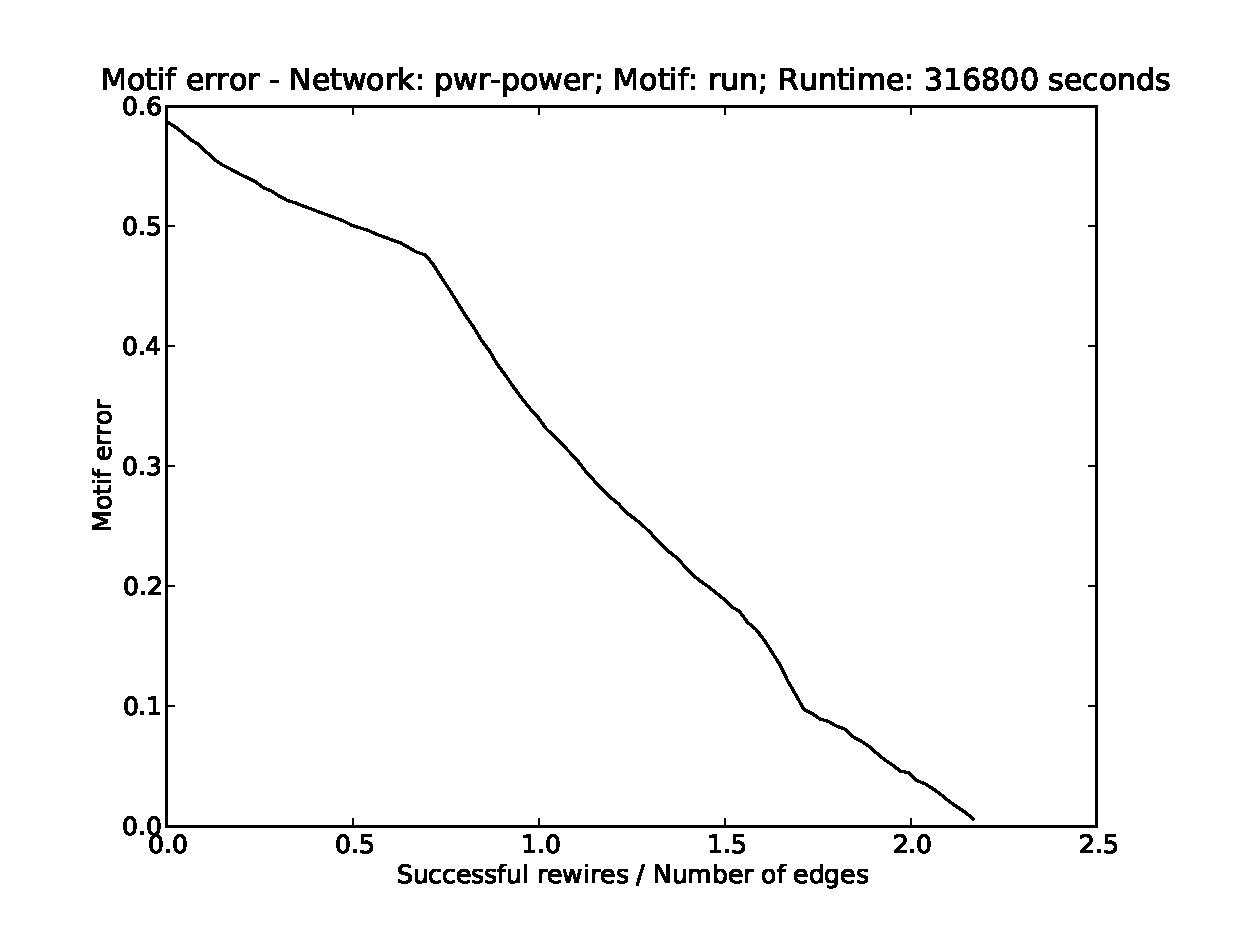
\includegraphics[width=3in]{Figures/motif_error-pwr-power-run.eps}
\caption{Experiment 2, network pwr-power.}
\label{fig:exp2-pwr-power-run}
\end{figure}

\begin{figure}[p]
\centering
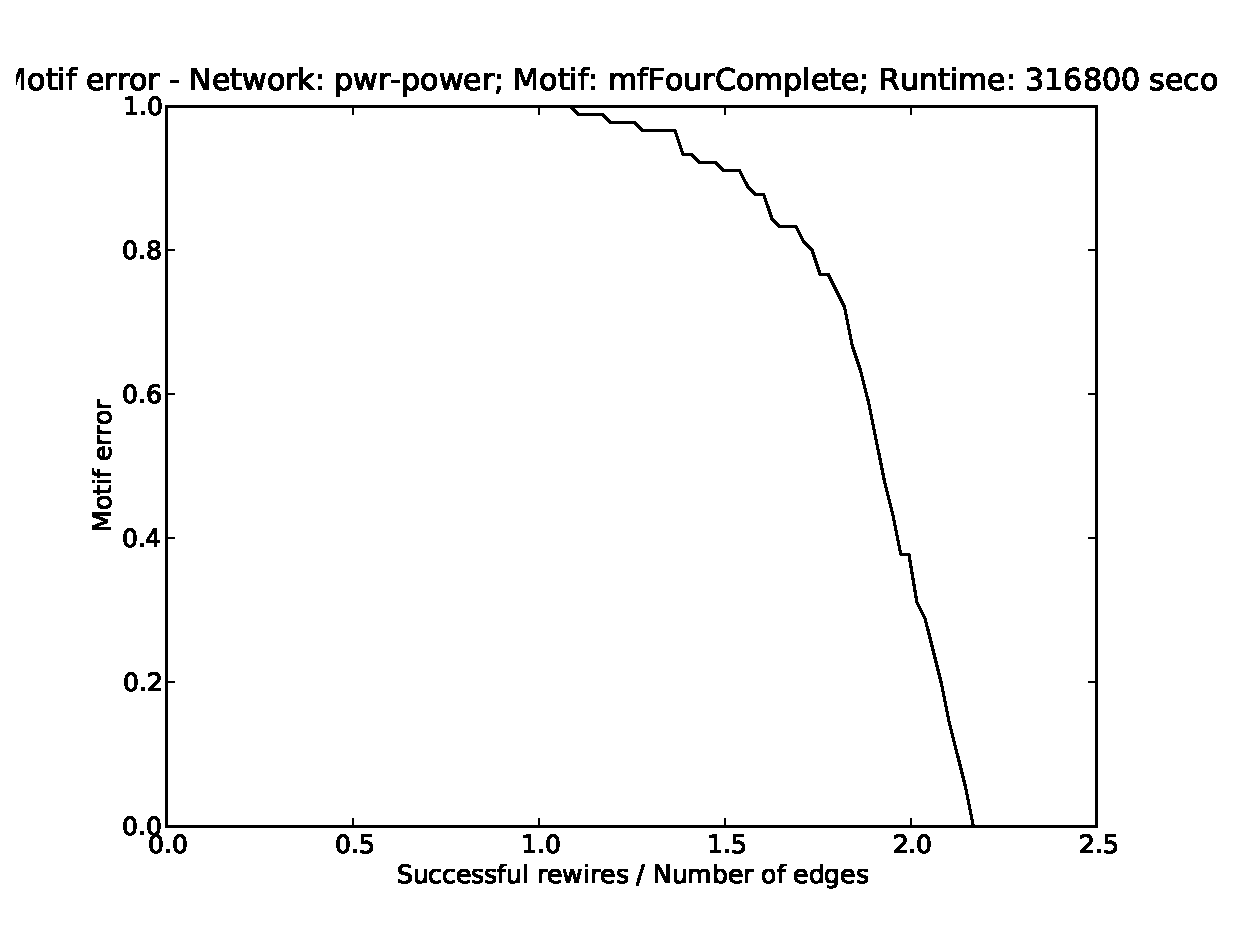
\includegraphics[width=3in]{Figures/motif_error-pwr-power-mfFourComplete.eps}
\caption{Experiment 2, network pwr-power, motif mfFourComplete.}
\label{fig:exp2-pwr-power-mfFourComplete}
\end{figure}

\begin{figure}[p]
\centering
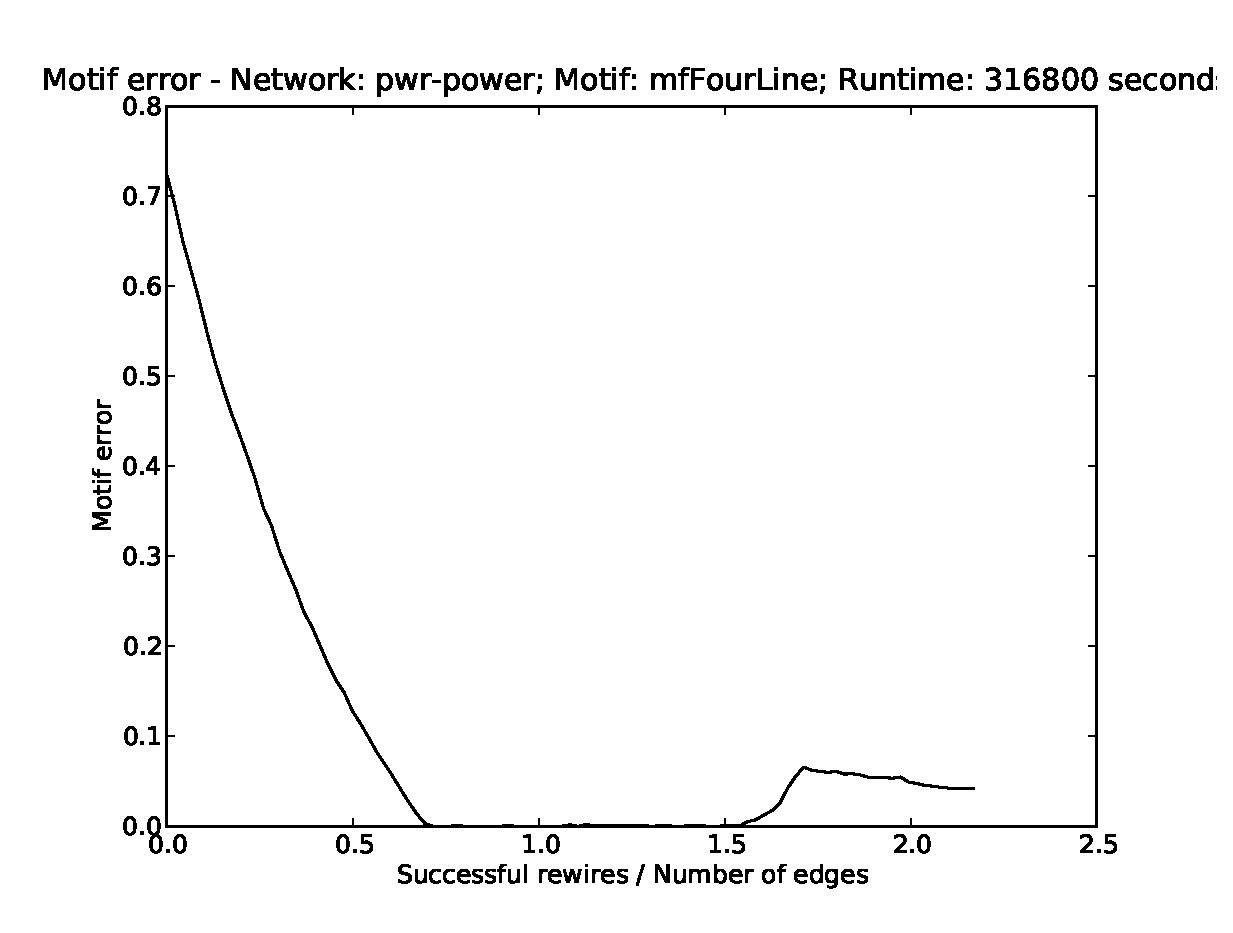
\includegraphics[width=3in]{Figures/motif_error-pwr-power-mfFourLine.eps}
\caption{Experiment 2, network pwr-power, motif mfFourLine.}
\label{fig:exp2-pwr-power-mfFourLine}
\end{figure}

\begin{figure}[p]
\centering
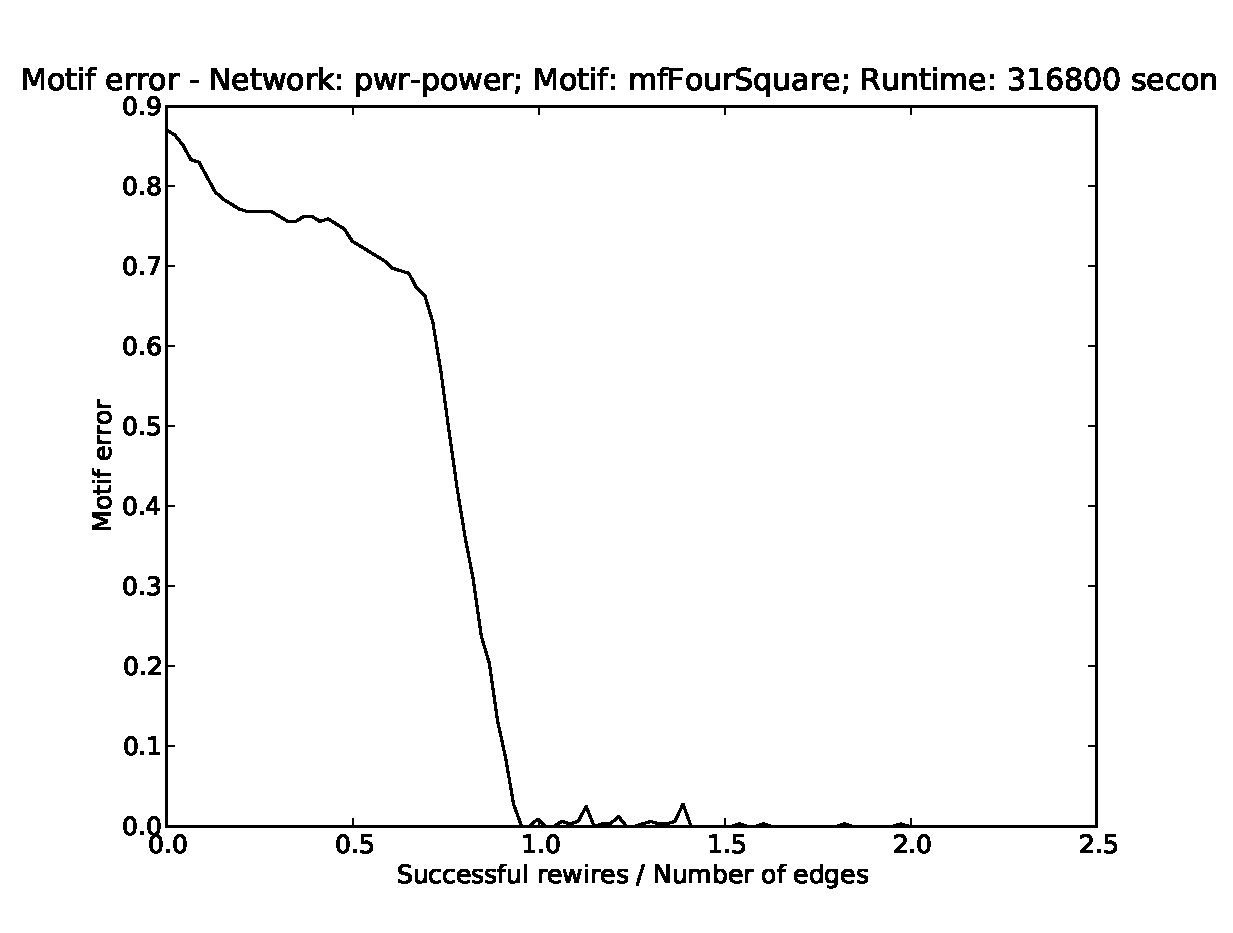
\includegraphics[width=3in]{Figures/motif_error-pwr-power-mfFourSquare.eps}
\caption{Experiment 2, network pwr-power, motif mfFourSquare.}
\label{fig:exp2-pwr-power-mfFourSquare}
\end{figure}

\begin{figure}[p]
\centering
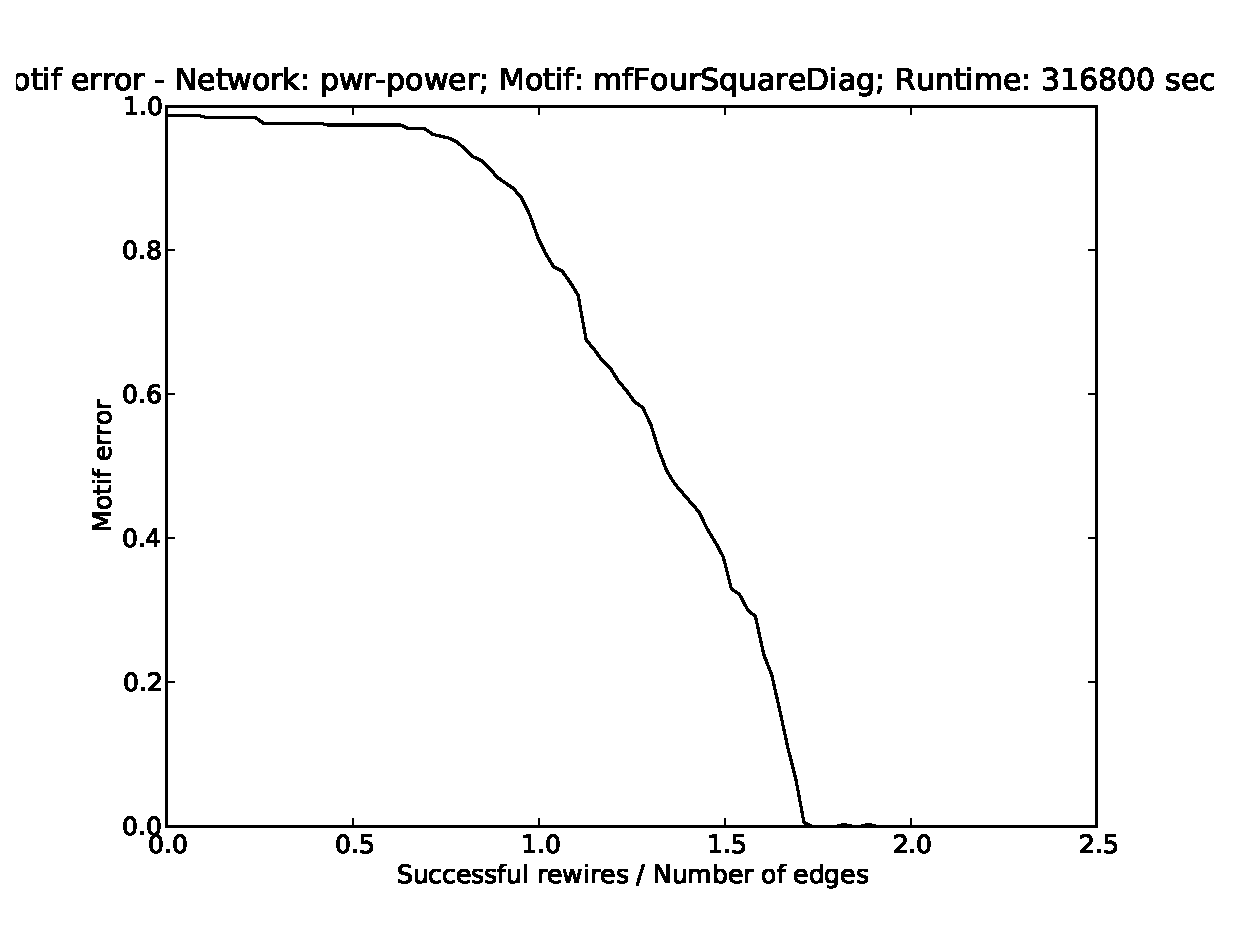
\includegraphics[width=3in]{Figures/motif_error-pwr-power-mfFourSquareDiag.eps}
\caption{Experiment 2, network pwr-power, motif mfFourSquareDiag.}
\label{fig:exp2-pwr-power-mfFourSquareDiag}
\end{figure}

\begin{figure}[p]
\centering
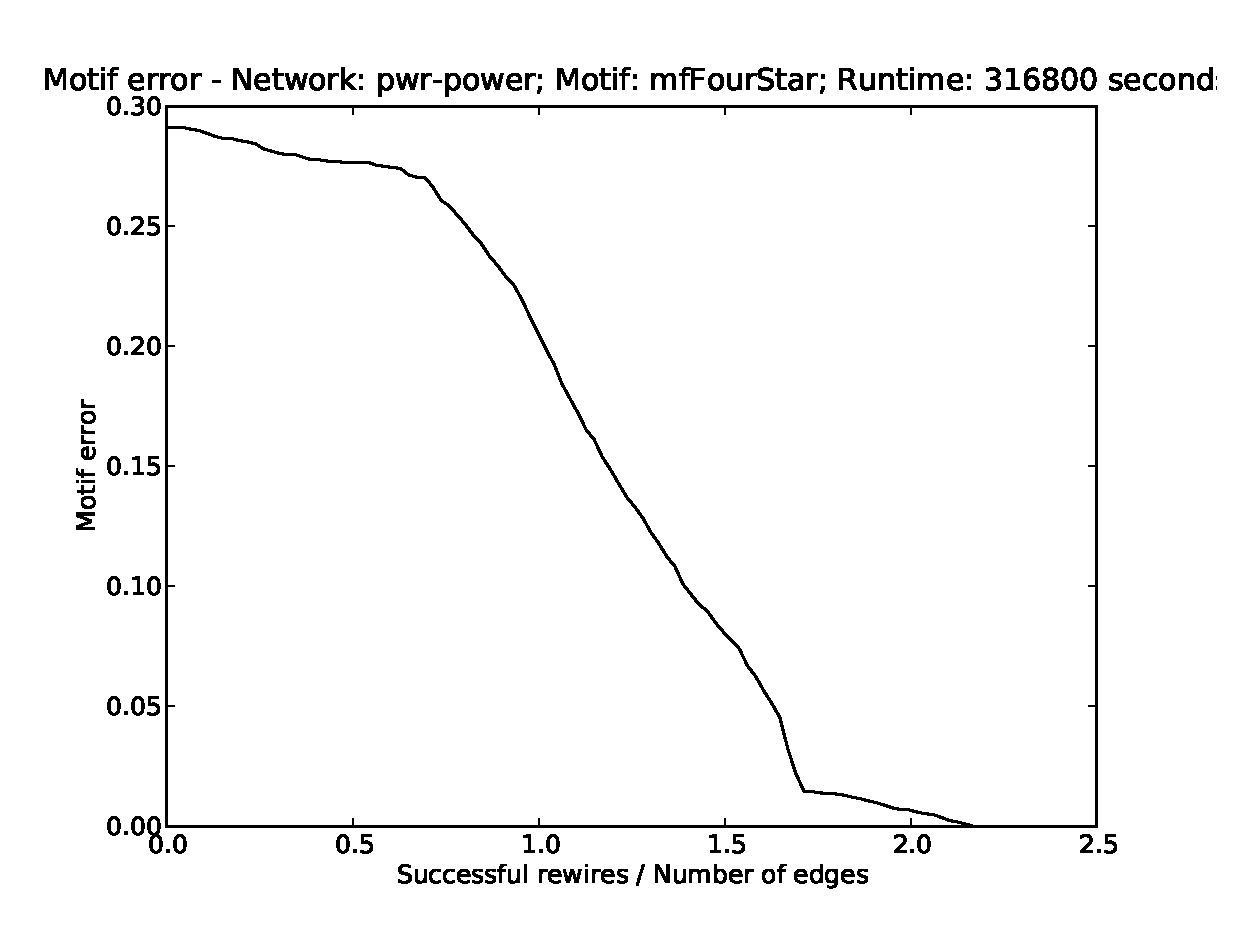
\includegraphics[width=3in]{Figures/motif_error-pwr-power-mfFourStar.eps}
\caption{Experiment 2, network pwr-power, motif mfFourStar.}
\label{fig:exp2-pwr-power-mfFourStar}
\end{figure}

\begin{figure}[p]
\centering
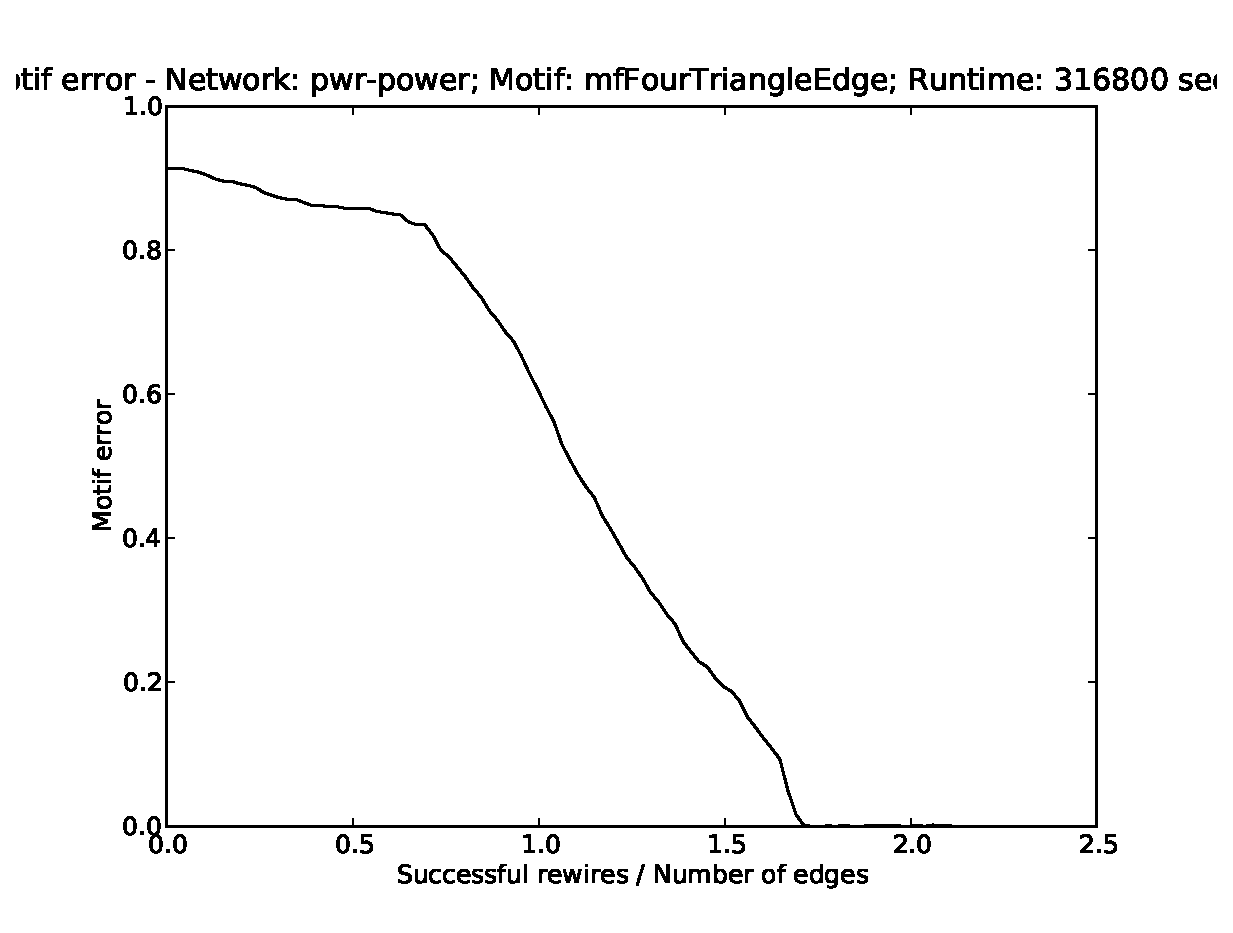
\includegraphics[width=3in]{Figures/motif_error-pwr-power-mfFourTriangleEdge.eps}
\caption{Experiment 2, network pwr-power, motif mfFourTriangleEdge.}
\label{fig:exp2-pwr-power-mfFourTriangleEdge}
\end{figure}

\begin{figure}[p]
\centering
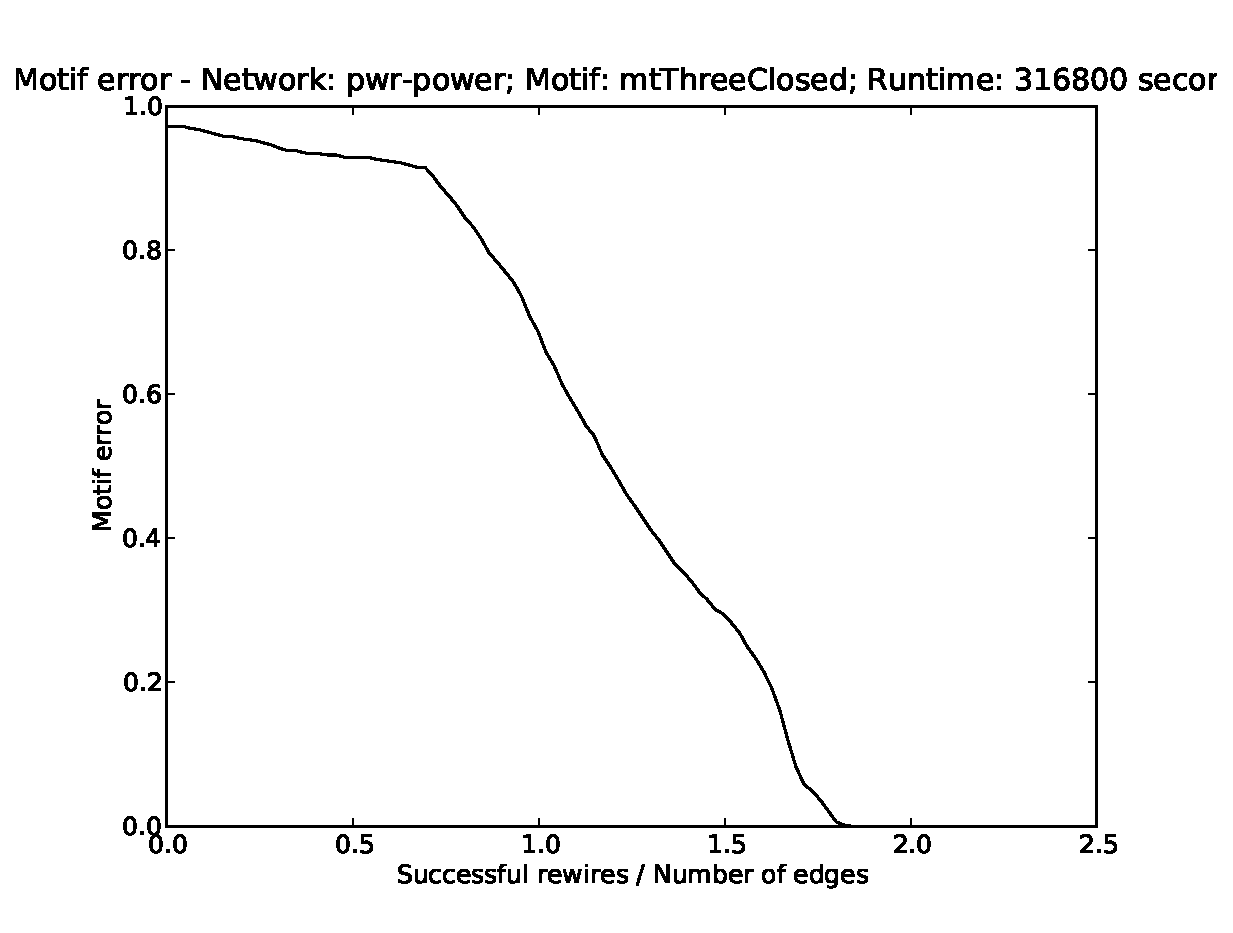
\includegraphics[width=3in]{Figures/motif_error-pwr-power-mtThreeClosed.eps}
\caption{Experiment 2, network pwr-power, motif mtThreeClosed.}
\label{fig:exp2-pwr-power-mtThreeClosed}
\end{figure}

\begin{figure}[p]
\centering
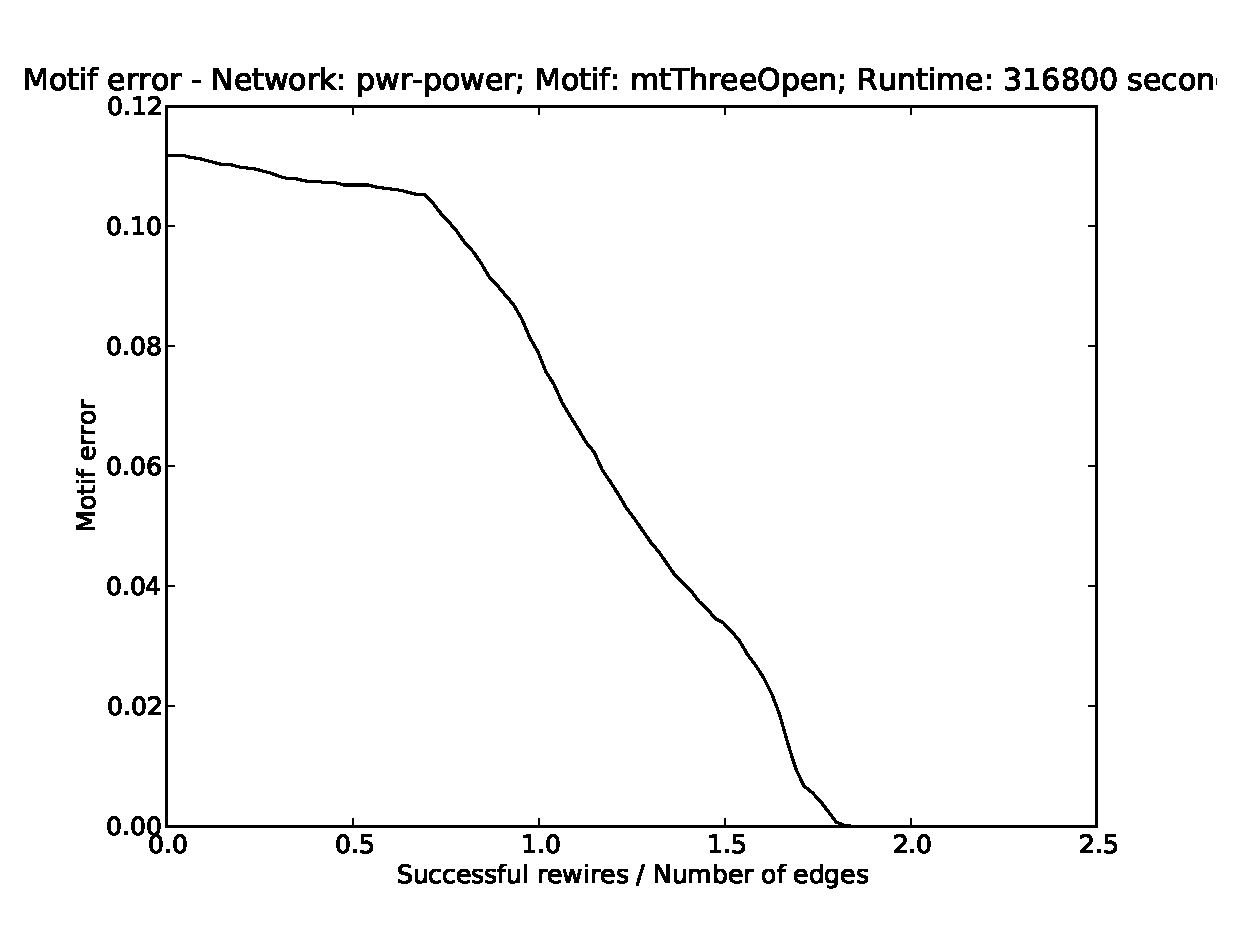
\includegraphics[width=3in]{Figures/motif_error-pwr-power-mtThreeOpen.eps}
\caption{Experiment 2, network pwr-power, motif mtThreeOpen.}
\label{fig:exp2-pwr-power-mtThreeOpen}
\end{figure}

%\begin{figure}[p]
%\centering
%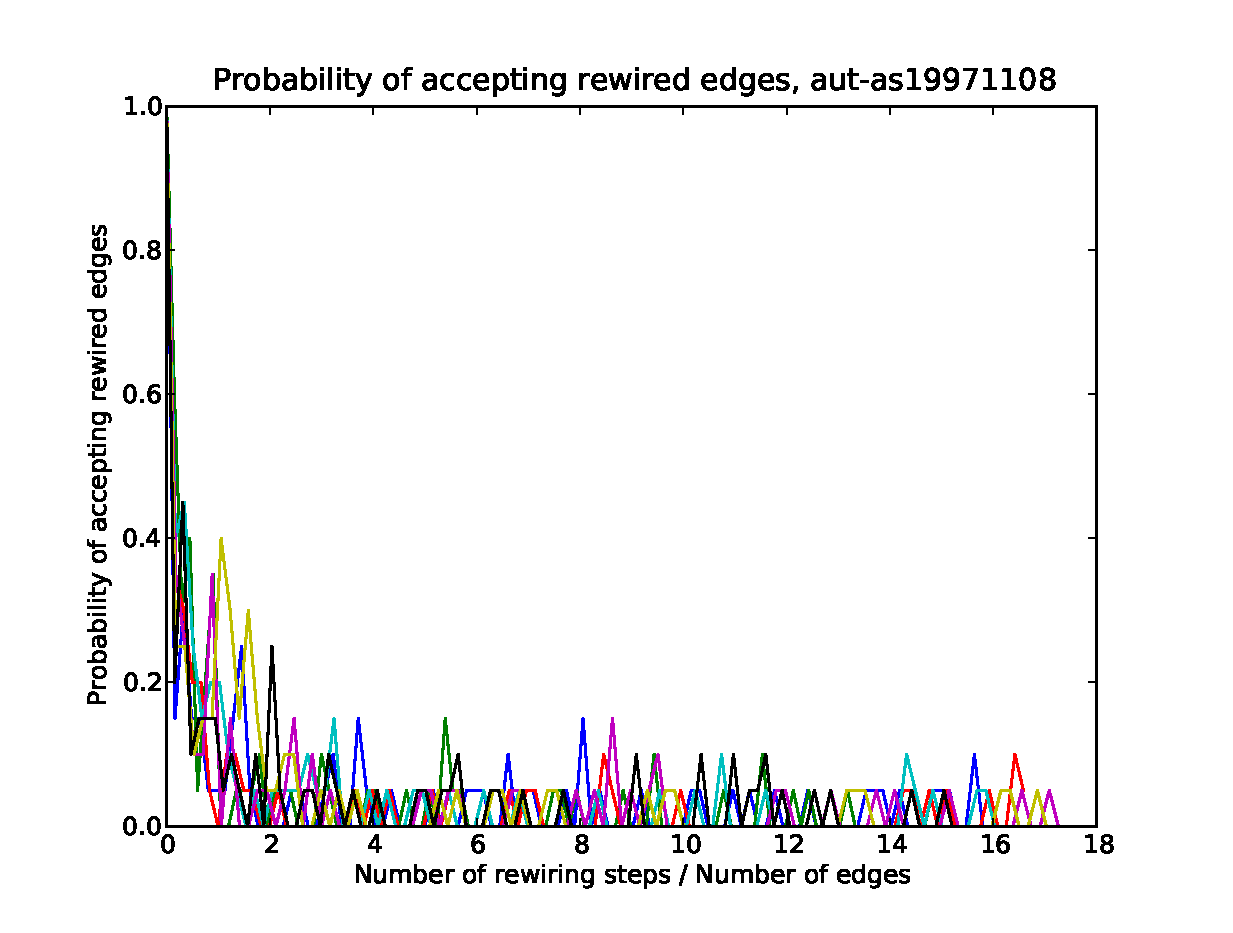
\includegraphics[width=3in]{Figures/Paccept-aut-as19971108.eps}
%\caption{Probability of a rewiring step being successful, network aut-as19971108}
%\label{fig:Paccept-aut-as19971108}
%\end{figure}
%
%\begin{figure}[p]
%\centering
%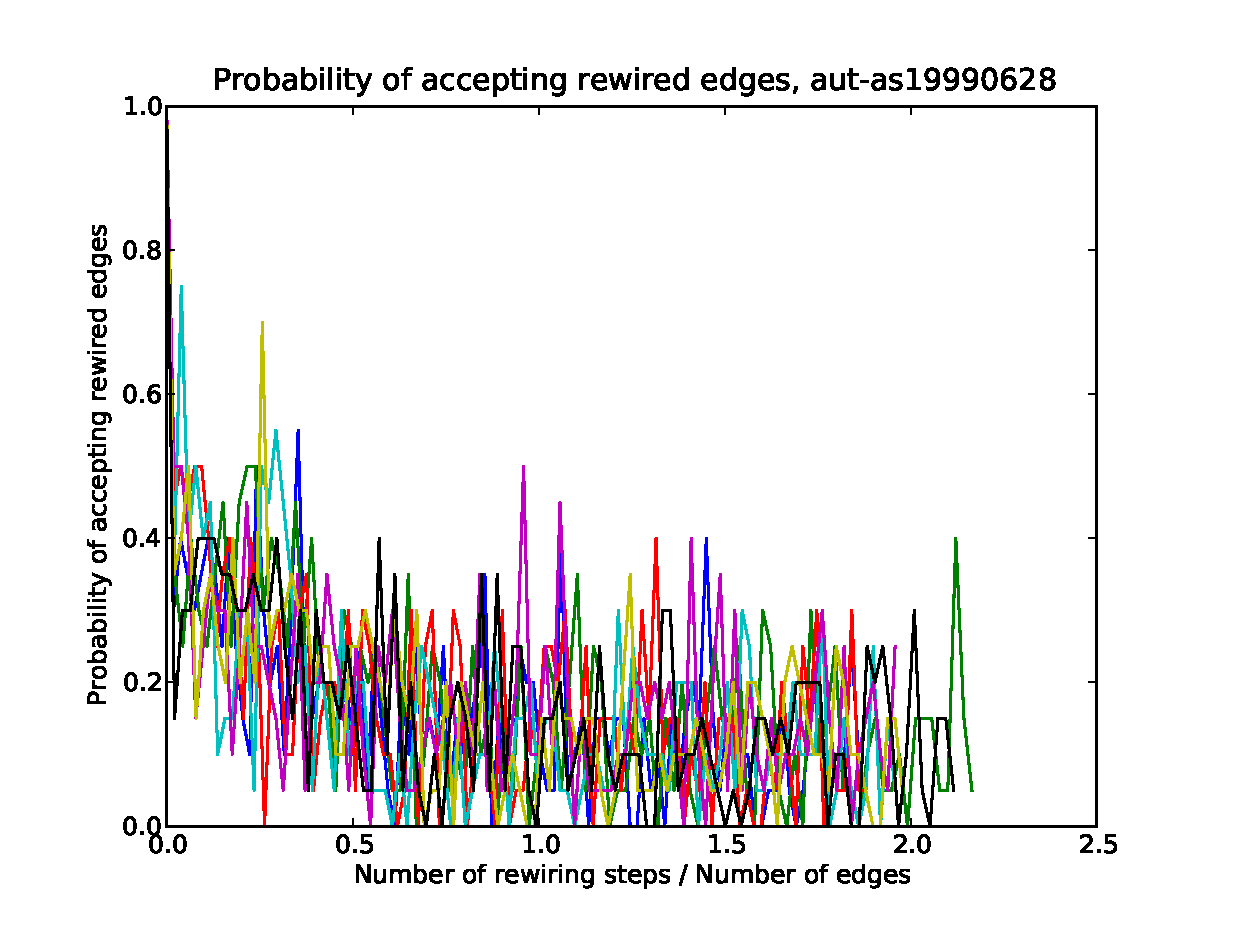
\includegraphics[width=3in]{Figures/Paccept-aut-as19990628.eps}
%\caption{Probability of a rewiring step being successful, network aut-as19990628}
%\label{fig:Paccept-aut-as19990628}
%\end{figure}
%
%\begin{figure}[p]
%\centering
%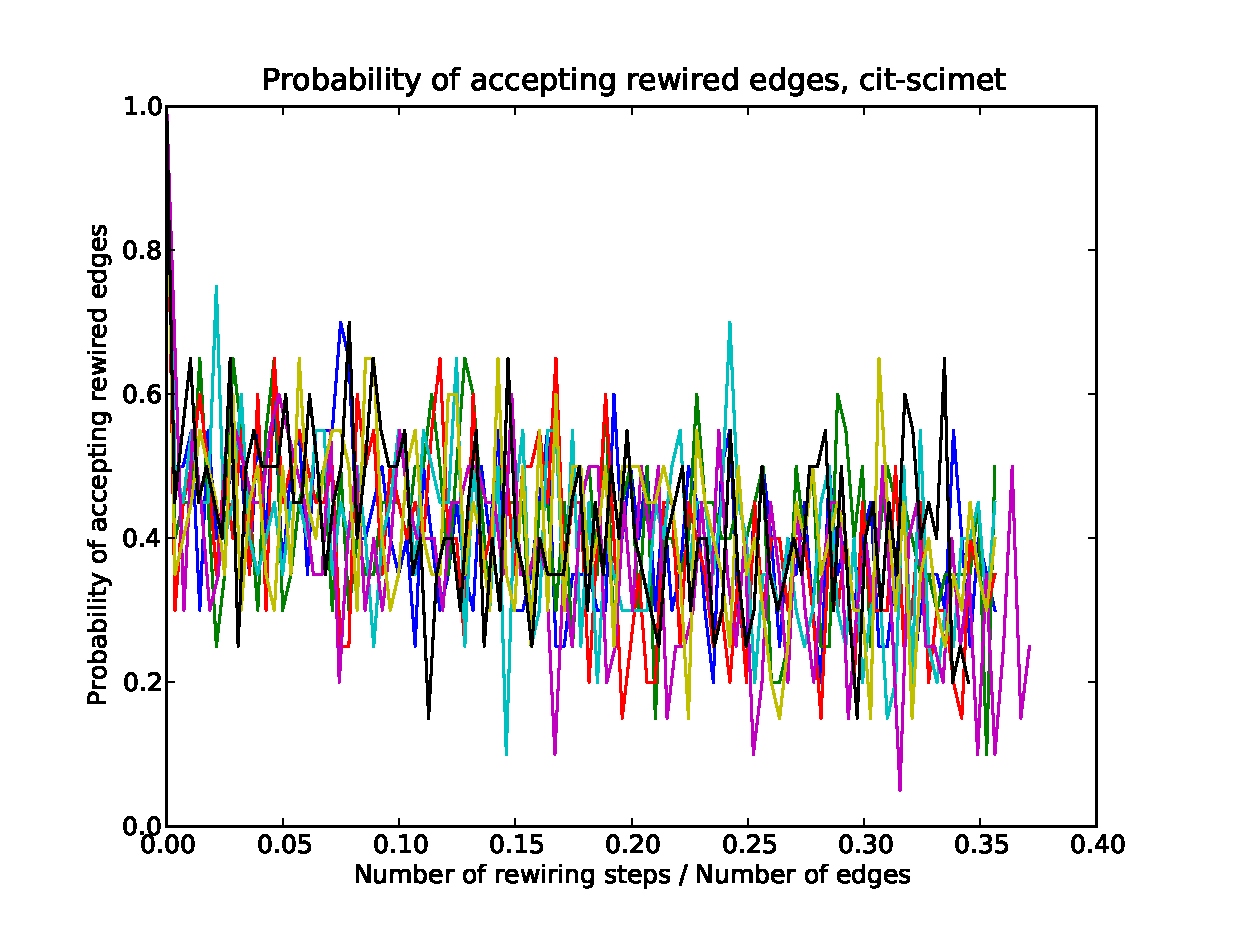
\includegraphics[width=3in]{Figures/Paccept-cit-scimet.eps}
%\caption{Probability of a rewiring step being successful, network cit-scimet}
%\label{fig:Paccept-cit-scimet}
%\end{figure}
%
%\begin{figure}[p]
%\centering
%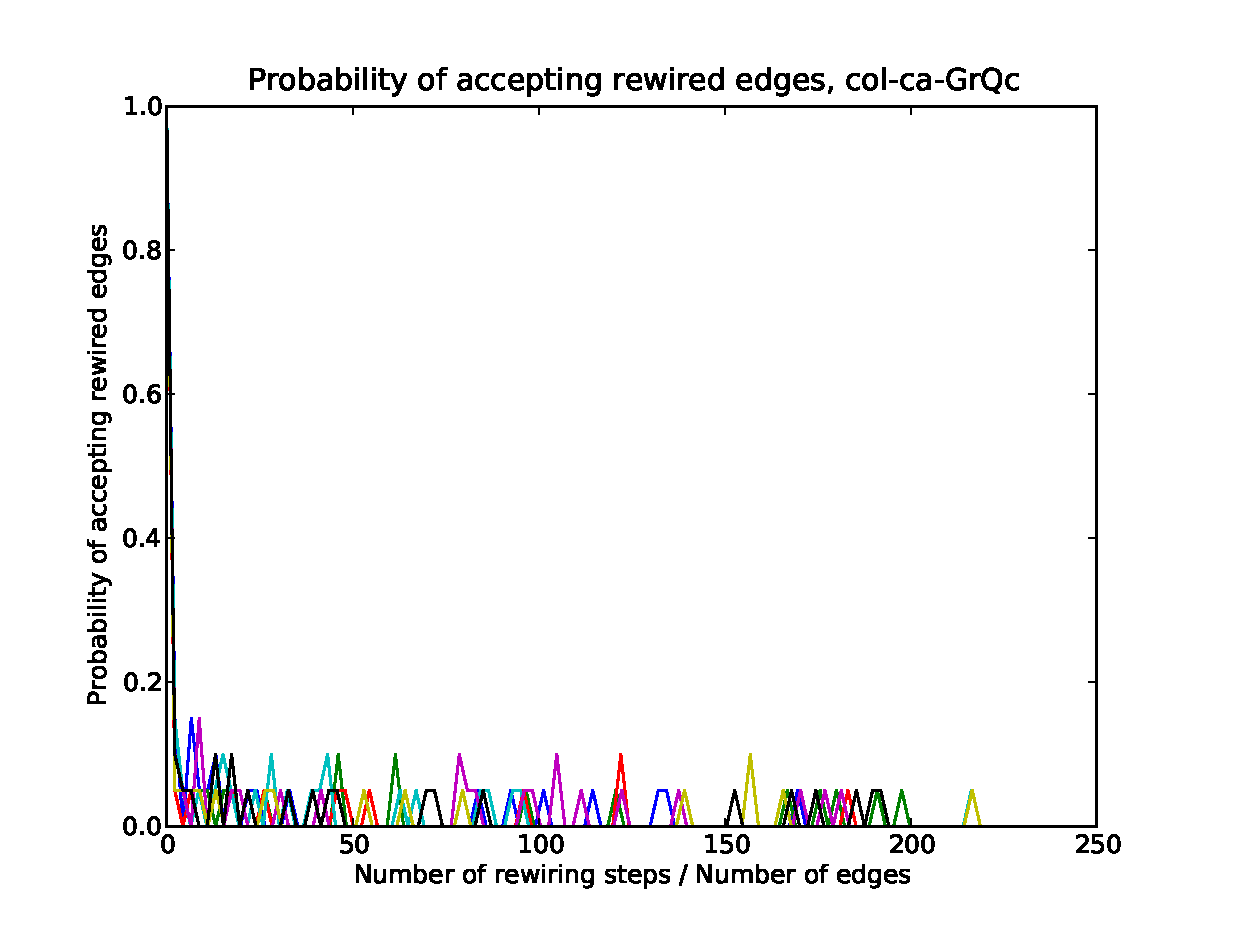
\includegraphics[width=3in]{Figures/Paccept-col-ca-GrQc.eps}
%\caption{Probability of a rewiring step being successful, network col-ca-GrQc}
%\label{fig:Paccept-col-ca-GrQc}
%\end{figure}
%
%\begin{figure}[p]
%\centering
%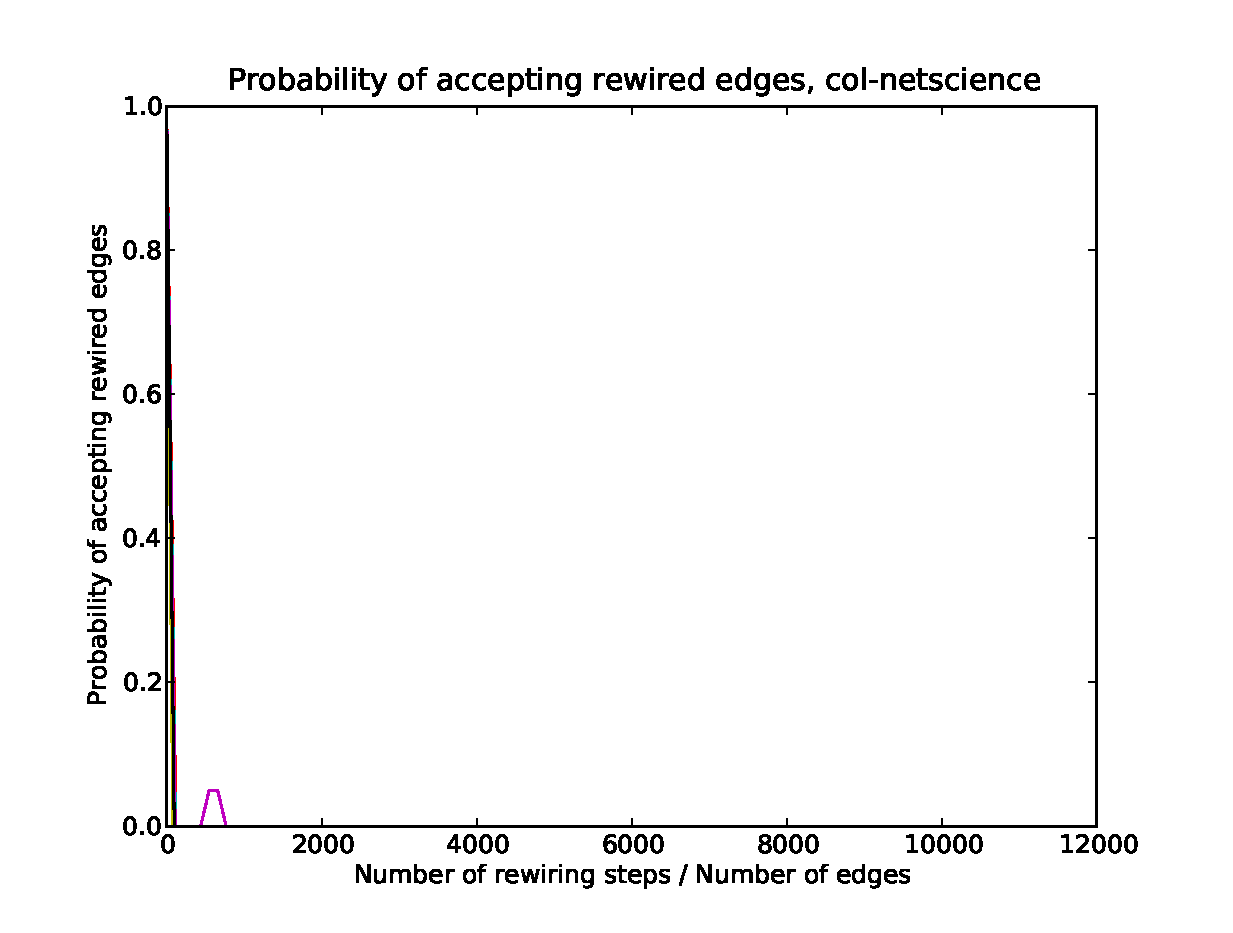
\includegraphics[width=3in]{Figures/Paccept-col-netscience.eps}
%\caption{Probability of a rewiring step being successful, network col-netscience}
%\label{fig:Paccept-col-netscience}
%\end{figure}
%
%\begin{figure}[p]
%\centering
%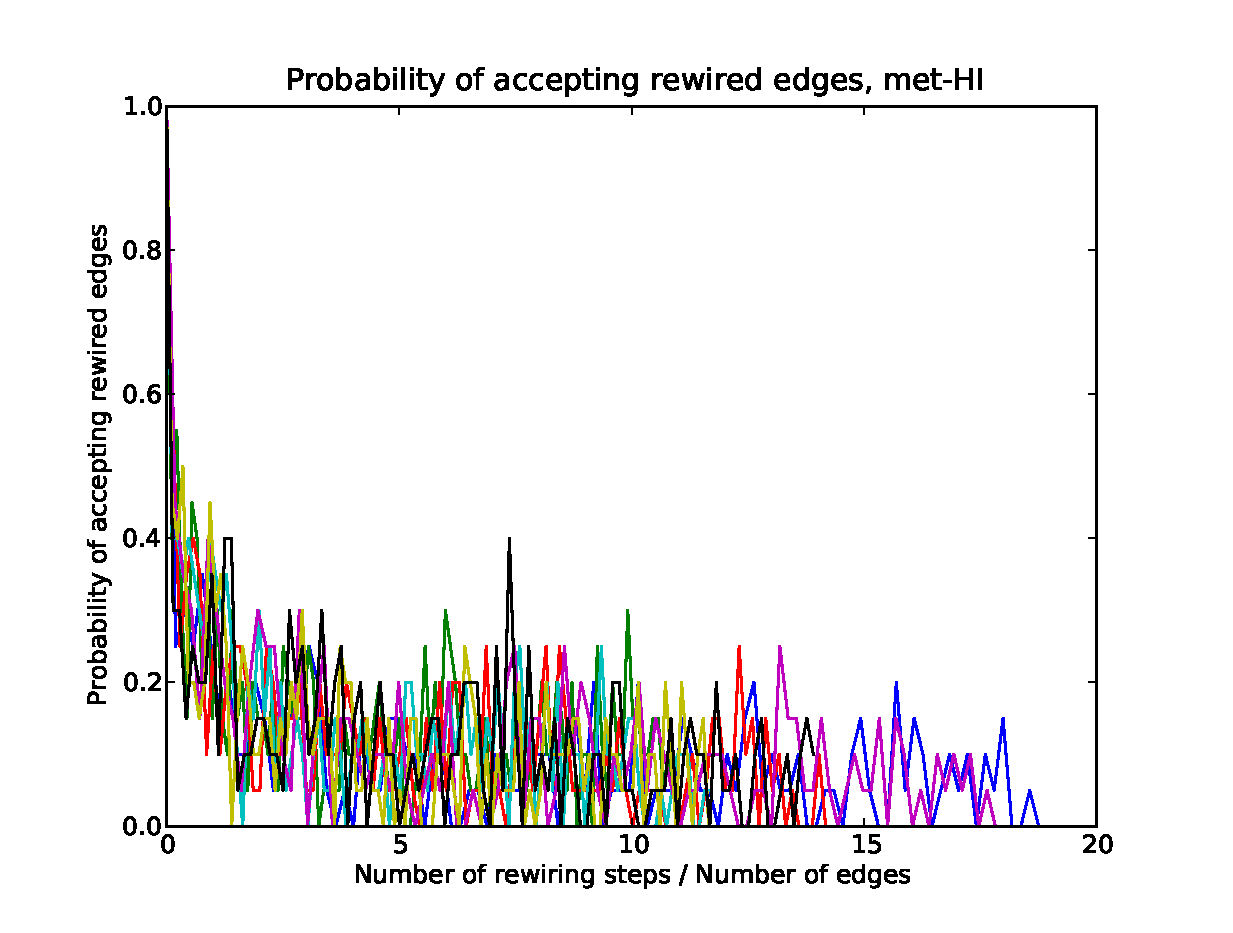
\includegraphics[width=3in]{Figures/Paccept-met-HI.eps}
%\caption{Probability of a rewiring step being successful, network met-HI}
%\label{fig:Paccept-met-HI}
%\end{figure}
%
%\begin{figure}[p]
%\centering
%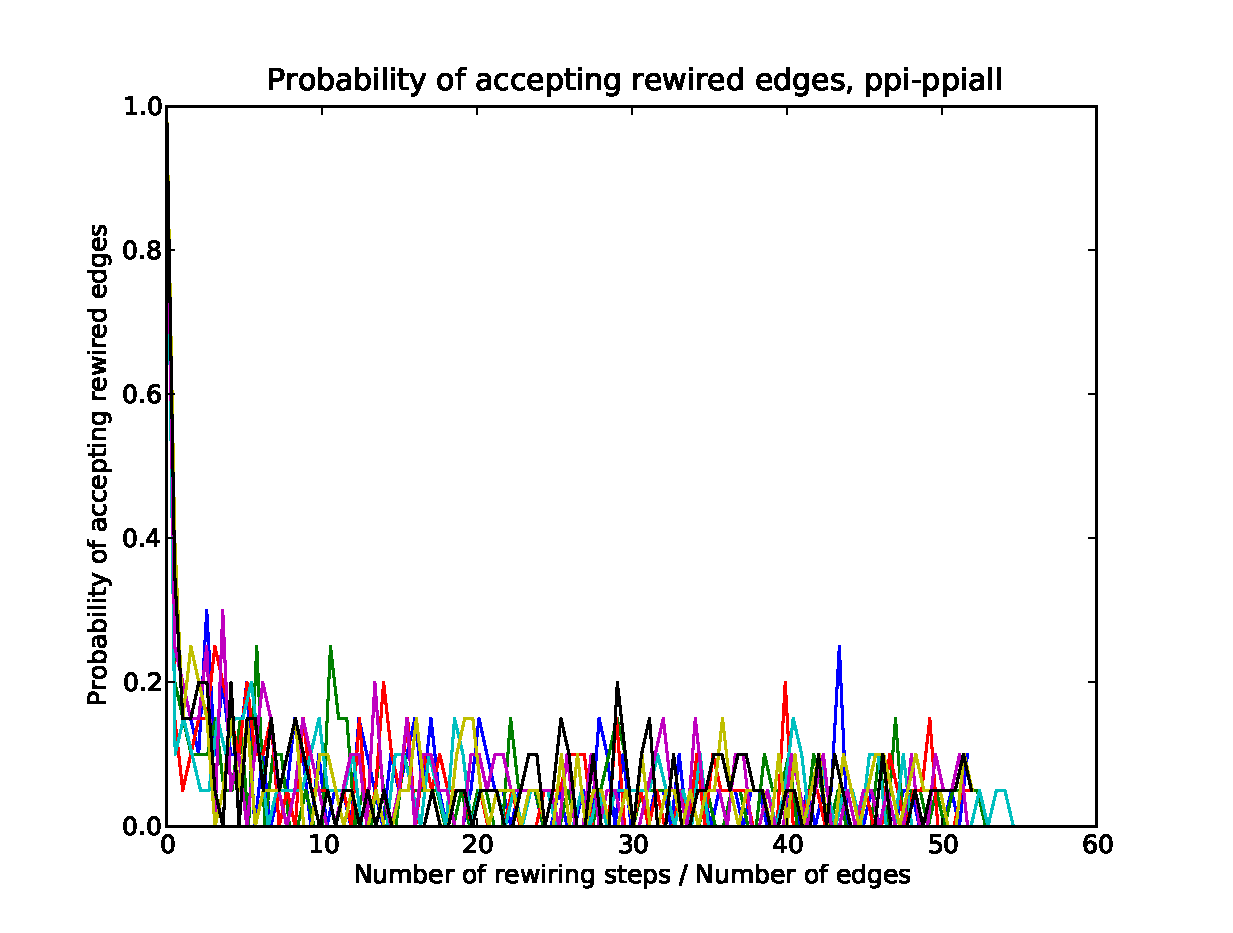
\includegraphics[width=3in]{Figures/Paccept-ppi-ppiall.eps}
%\caption{Probability of a rewiring step being successful, network ppi-ppiall}
%\label{fig:Paccept-ppi-ppiall}
%\end{figure}
%
%\begin{figure}[p]
%\centering
%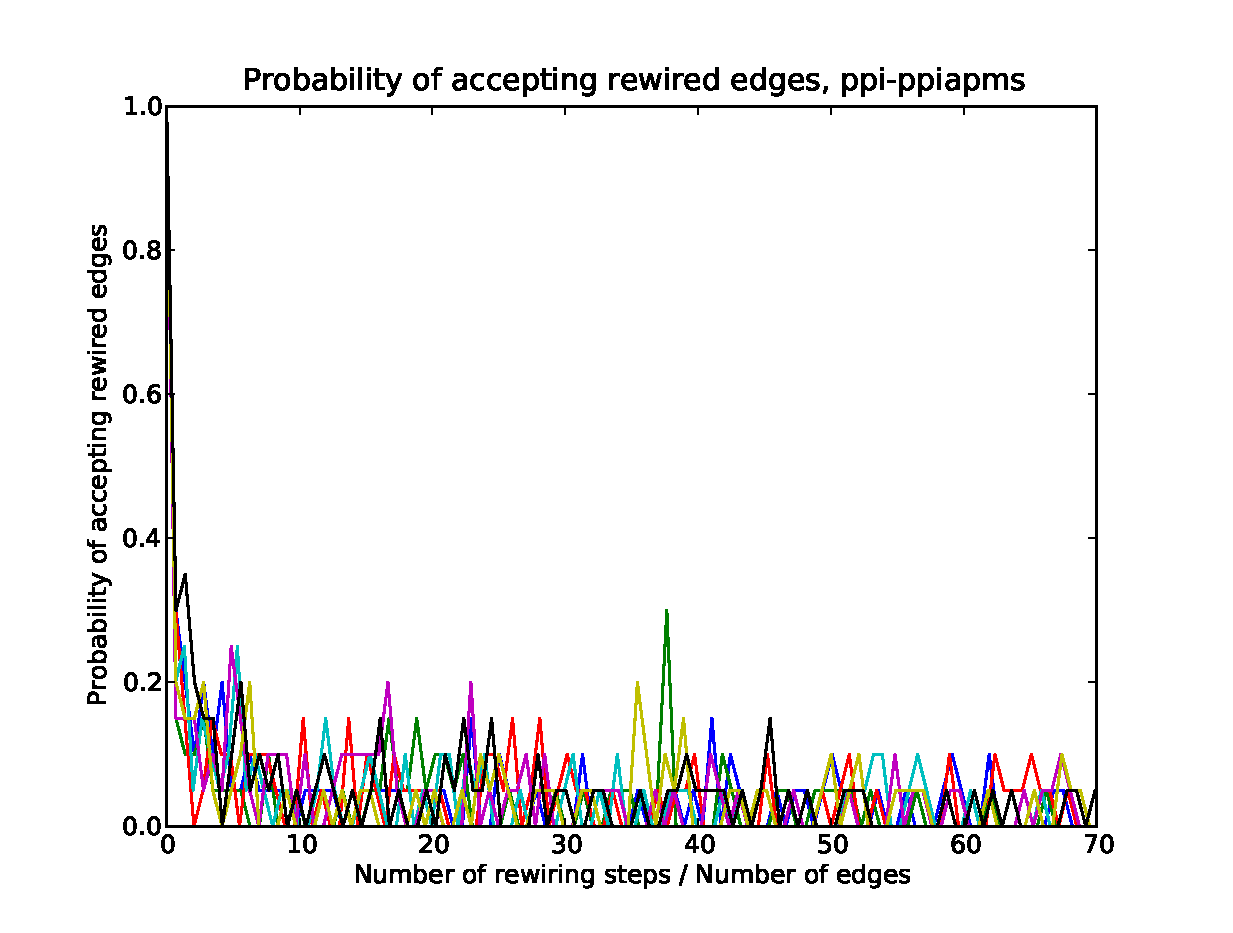
\includegraphics[width=3in]{Figures/Paccept-ppi-ppiapms.eps}
%\caption{Probability of a rewiring step being successful, network ppi-ppiapms}
%\label{fig:Paccept-ppi-ppiapms}
%\end{figure}
%
%\begin{figure}[p]
%\centering
%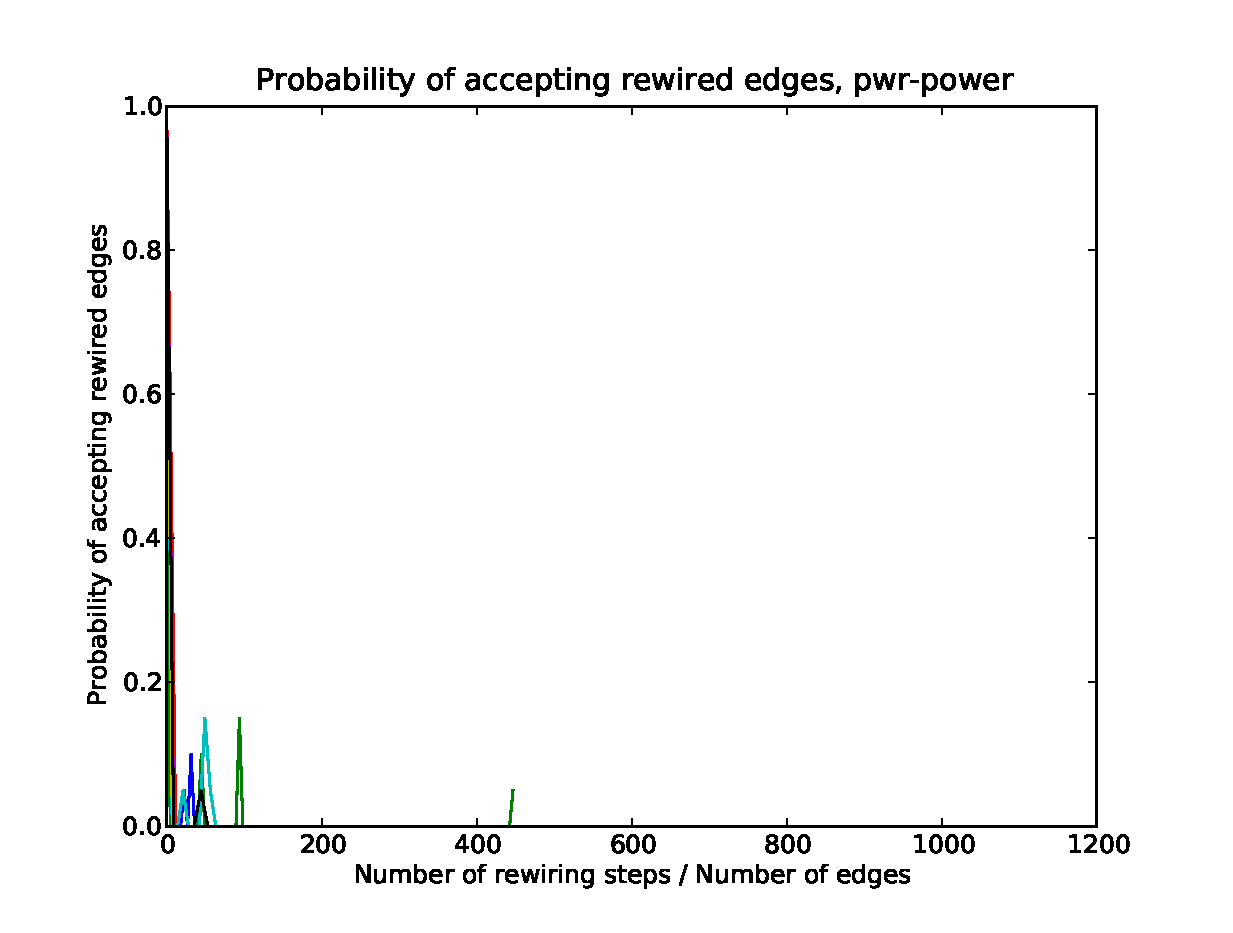
\includegraphics[width=3in]{Figures/Paccept-pwr-power.eps}
%\caption{Probability of a rewiring step being successful, network pwr-power}
%\label{fig:Paccept-pwr-power}
%\end{figure}
